\chapter{Experimentación}

% ------------------------------------------------------------------------------------------------------------
% ------------------------------------------------------------------------------------------------------------

\section{Protocolo de validación experimental}

Como se ha comentado anteriormente, se han proporcionado los datos ya dividos en conjunto de entrenamiento (\textit{train}) y de test, para evitar problemas asociados al \textit{data snooping}%
\footnote{
    El \textbf{\textit{data snooping}} ocurre cuando información del conjunto de test se filtra, directa o indirectamente, en el proceso de entrenamiento del modelo, lo que puede llevar a una sobreestimación del rendimiento y a modelos que no generalizan adecuadamente ante datos nuevos.
}.
Al proporcionar las particiones predefinidas, se garantiza que no haya contaminación entre los datos de entrenamiento y test, manteniendo así la validez de las métricas obtenidas en el test. 

Sin embargo, si se optimizan los parámetros del modelo durante el entrenamiento sin disponer de un conjunto independiente para evaluar su rendimiento, se corre el riesgo de sobreajustarse a los datos de entrenamiento. Es por ello que, además del conjunto de entrenamiento y test, es esencial tener un \textbf{conjunto de validación} independiente que permita evaluar el modelo durante su desarrollo, ajustar hiperparámetros y comparar diferentes configuraciones sin contaminar la evaluación final en el conjunto de test. Se consideró realizar validación cruzada (\textit{cross-validation}), pero debido al elevado coste computacional que implica, los resultados satisfactorios obtenidos mediante una simple partición de los datos (\textit{train/validation split}), se decidió prescindir de su aplicación.

En la Figura \ref{fig:data_split_base} podemos ver la división del \textit{dataset} planteada. Cabe comentar que la división se ha realizado de forma estratificada en base a la edad y el sexo%
\footnote{
    La estratificación se realizó en intervalos de medio año de edad y por sexo; por ejemplo, una instancia con edad 17.7 y sexo masculino se etiquetó como ``17.5\_M''.
}.

\begin{figure}[h]
    \centering
    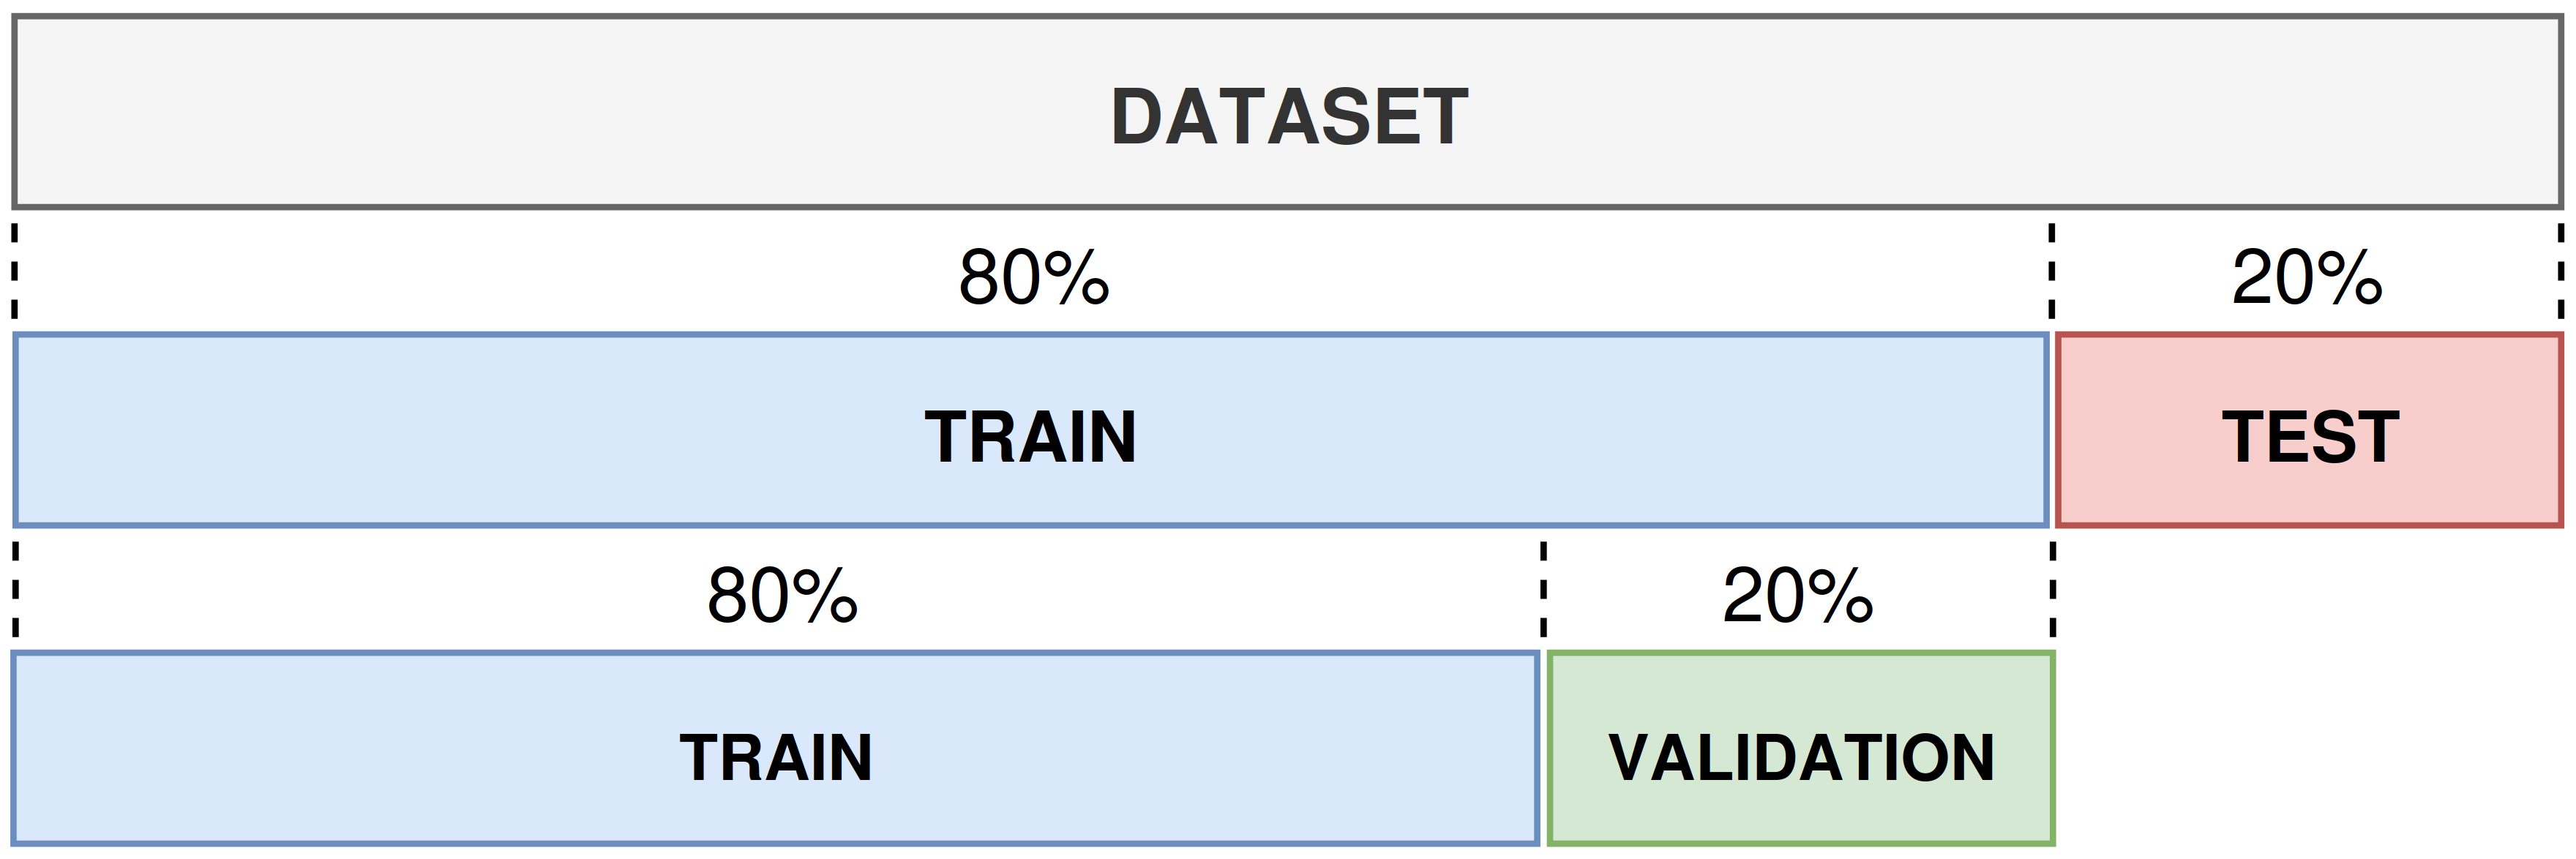
\includegraphics[width=0.8\textwidth]{capitulos/cap_04/imagenes/data_split_base.png}
    \caption[
        Diagrama de división del \textit{dataset} en \textit{train}, \textit{validation} y \textit{test}.
    ]{
        Diagrama de división del \textit{dataset} en \textit{train}, \textit{validation} y \textit{test}. 
    } 
    \label{fig:data_split_base}
\end{figure}

Es importante destacar que esta división se mantiene constante en todos los experimentos y para todos los problemas planteados, asegurando que las mismas instancias permanezcan en los mismos subconjuntos. Esto permite garantizar que ningún modelo preentrenado reutilice datos previamente utilizados en etapas de validación o calibración, algo especialmente relevante dado que los problemas abordados están jerárquicamente relacionados (la clasificación de sexo y mayoría de edad se deriva directamente de la clasificación de mayoría de edad, que a su vez se deriva de la estimación de edad).

Sin embargo, al emplear métodos de calibración o predicción conformal, si usamos los mismos datos de entrenamiento para la calibración, las probabilidades o intervalos de predicción tenderán a ser optimistas, pues el modelo ha sido entrenado con esos datos \cite{niculescu2005}. Por tanto, para evitar el sobreajuste y garantizar validez estadística se requiere de un subconjunto de datos adicional: el \textbf{conjunto de calibración}. Se ha escogido destinar el  20\% de los ejemplos de entrenamiento para calibración, basándose en los resultados empíricos de \cite{sesia2020} (que recomienda dedicar entre un 10\% y 30\% de datos de entrenamiento a calibración), tal y como se muestra en la Figura \ref{fig:data_split_conformal}.

\begin{figure}[h]
    \centering
    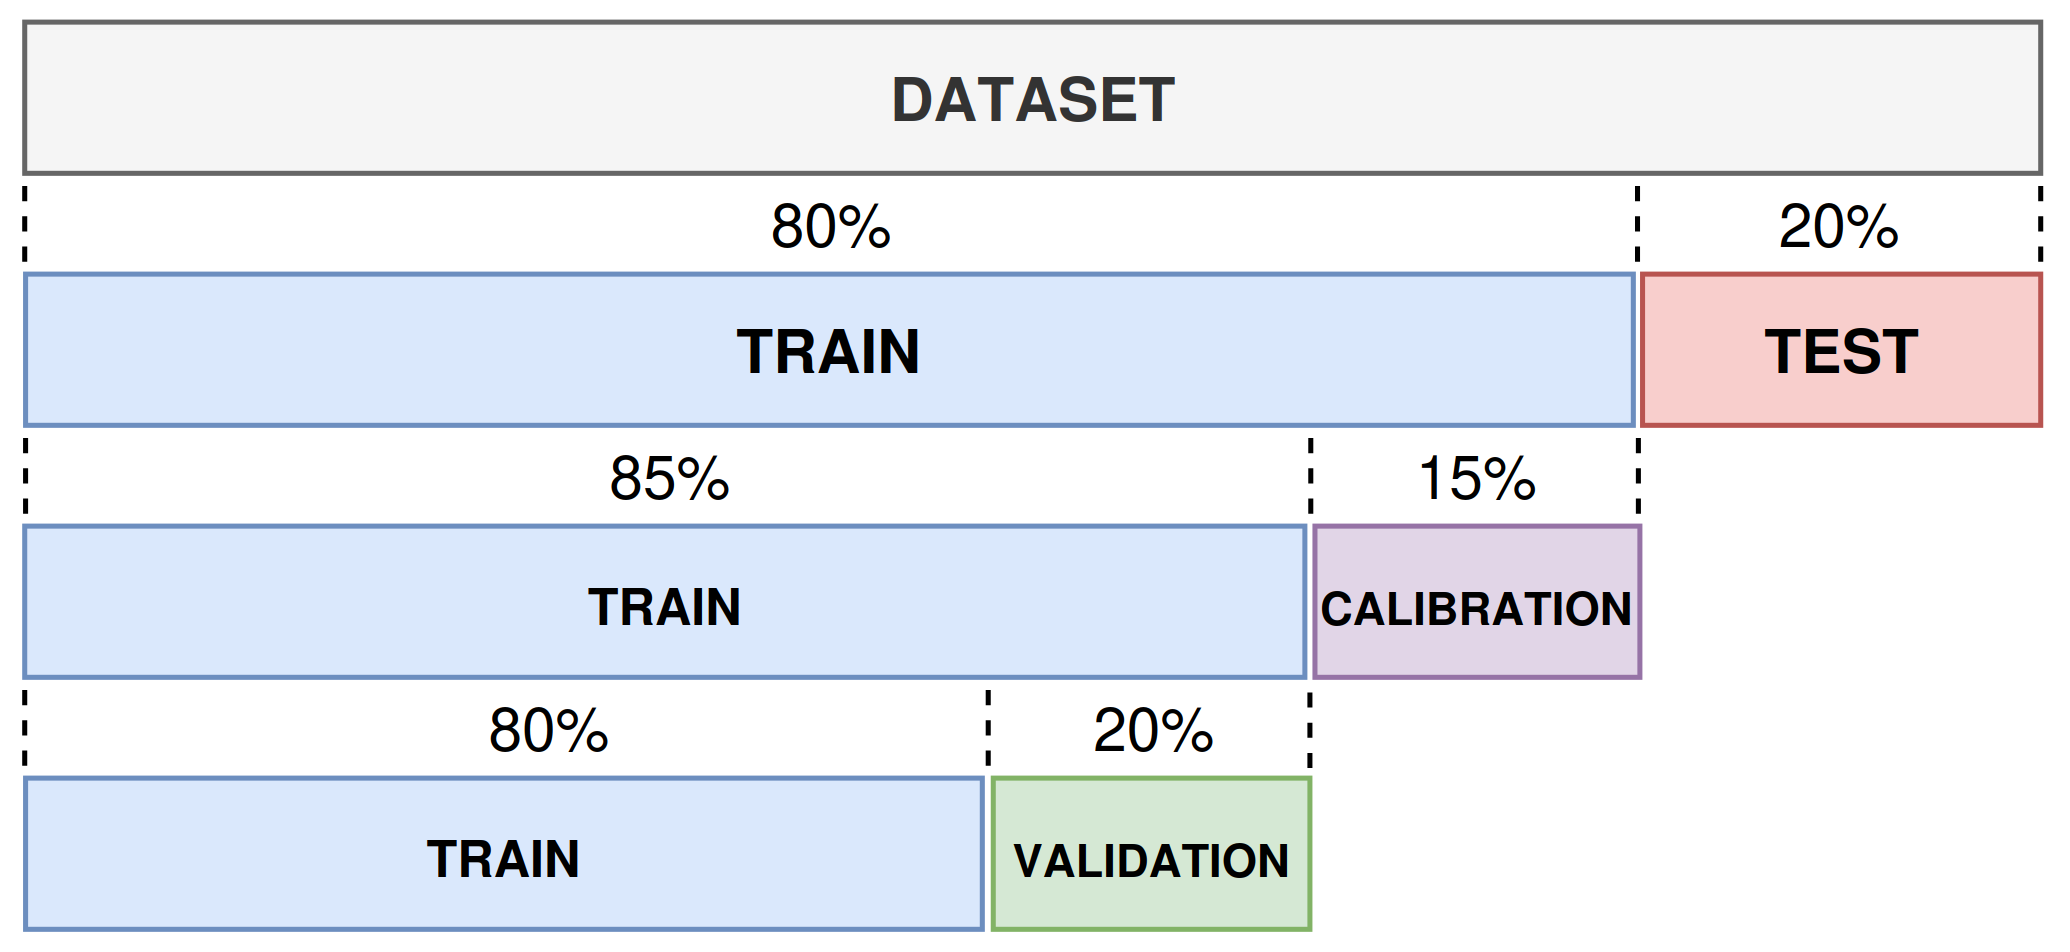
\includegraphics[width=0.8\textwidth]{capitulos/cap_04/imagenes/data_split_conformal.png}
    \caption[
        Diagrama de división del \textit{dataset} en \textit{train}, \textit{validation}, \textit{calibration} y \textit{test}.
    ]{
        Diagrama de división del \textit{dataset} en \textit{train}, \textit{validation}, \textit{calibration} y \textit{test}. 
    } 
    \label{fig:data_split_conformal}
\end{figure}

Para una comparativa más justa entre los métodos que usan CP y los que no, se utilizará la siguiente estrategia: los métodos que no emplean CP seguirán el esquema tradicional de división de datos (en entrenamiento, validación y test), mientras que los métodos basados en CP incorporarán además un conjunto de calibración independiente. Esta diferencia en el diseño experimental nos permitirá cuantificar cómo afecta a la capacidad predictiva de los modelos el hecho de reservar parte de los datos para el proceso de calibración.

% ------------------------------------------------------------------------------------------------------------
% ------------------------------------------------------------------------------------------------------------

\section{Experimentos propuestos}

% ------------------------------------------------------------------------------------------------------------

\subsection{Comparativa de métodos para la estimación de edad}

Se plantea una comparativa entre diversos métodos de predicción para el problema de AE. Todos los métodos presentan tanto predicción puntual como interválica. De esta forma queremos evaluar tanto su utilidad tradicional para estimar el valor esperado como su capacidad para proporcionar intervalos de confianza fiables que capturen la incertidumbre predictiva y sean computacionalmente eficientes. El objetivos es alcanzar el 95\% de confianza en las predicciones interválicas, que es la cifra de confianza generalmente empleada en AF. Los métodos propuestos son los siguientes: 

\begin{itemize}

    \item \textbf{Método `base'}: Se trata de un modelo de regresión puntual sin técnicas de CP. La predicción interválica se construirá con la predicción puntual $\pm$ 2 veces el error absoluto medio obtenido en el conjunto de validación, que es una aproximación heurística común para construir intervalos de predicción que no asumen una distribución de errores específica. Este método sirve como \textit{baseline} para comparar la mejora que aportan las técnicas más sofisticadas.

    \item \textbf{Método `ICP'}: Implementa el método ICP, mediante el cual se ...
    
    \item \textbf{Método `QR'}: Este modelo implementa QR. Utiliza tres cuantiles 
    $$
    [0.5, \alpha/2, 1-\alpha/2]
    $$ 
    para predecir la predicción puntual, límite inferior y límite superior, respectivamente.

    \item \textbf{Método `CQR'}: Este modelo implement

\end{itemize} 

Para cada método se ha entrenado 10 modelos independientes desde cero, con el objetivo de capturar la variabilidad inherente al proceso de entrenamiento. Todas las métricas se calculan sobre el conjunto de test, evaluando tanto predicciones puntuales como interválicas, para garantizar que la evaluación sea objetiva y no esté influenciada por ninguna etapa del entrenamiento o calibración. 

% ------------------------------------------------------------------------------------------------------------

\subsection{Comparativa de métodos para la estimación de mayoría de edad}

Todos los métodos propuestos para el problema de AAM presentan una predicción puntual (de una sola etiqueta), además de un conjunto de predicción, formado por una o más etiquetas. 

Los métodos propuestos son:

\begin{itemize}

\item \textbf{Método `base'}: Se trata del modelo de clasificación de una sola etiqueta sin uso de técnicas de CP. El conjunto de predicción se considerará aquel formado exclusivamente por la clase más probable. El entrenamiento de este modelo partirá de un modelo `base' ya entrenado para el problema de AE, al cual se realizará un \textit{fine-tuning} de la cabecera. Este método sirve de \textit{baseline} para comparar con el resto. 

\item \textbf{Método `LAC'}: Este método implementa la técnica LAC para CP. El entrenamiento del modelo partirá de un modelo ICP ya entrenado para regresión.

\item \textbf{Método `MCM'}: Este método implementa la técnica MCM para CP. El modelo será exactamente el mismo que el de LAC. Solo cambiará la calibración e inferencia conformal. 

\end{itemize} 

No se han implementado los otros métodos de clasificación APS y RAPS, puesto que no son aplicables directamente al caso de clasificación binaria.

En este caso, también se han obtenido 10 modelos indepenndientes para cada método, y las métricas se han calculado sobre el conjunto de test. 

% ------------------------------------------------------------------------------------------------------------

\subsection{Comparativas de métodos para la clasificación combinada de mayoría de edad y sexo}

Al igual que en el problema de AAM, para el problema de AMSC se ha seguido la misma lógica de evaluación, aplicando tanto predicción puntual como técnicas de CP para obtener conjuntos de predicción. 

\todo{
    No me gusta mucho usar estas siglas en el texto, no sé si debería directamente eliminarlas del trabajo o solo dejarlas para usar en los resultados (para tablas y gráficos, donde no cabe mucho texto)
}

En este caso, se ha empleado la técnica de calibración de probabilidades \textit{Platt Scaling} para ajustar las salidas del modelo de clasificación multiclase, con el objetivo de mejorar la calidad de las probabilidades utilizadas durante la fase de inferencia conformal. Esta calibración probabilística se realiza antes de aplicar los métodos de CP. Se ha optado por utilizar el conjunto de validación para llevar a cabo dicha calibración de probabilidades, dado que, aunque no es el enfoque más riguroso ---ya que lo ideal sería dividir el conjunto de calibración en dos subconjuntos independientes, uno para la calibración de probabilidades y otro para la calibración conformal--- esta estrategia mostró buenos resultados en la práctica. Esto se debe a que el conjunto de validación empleado era suficientemente representativo y permitió obtener probabilidades calibradas de manera adecuada. Esta calibración probabilística no afecta a la variabilidad entre modelos con los mismos pesos, dado que el algoritmo es determinista y produce resultados consistentes para un mismo conjunto de datos y parámetros. 

Partiendo de esto, los métodos propuestos son:

\begin{itemize}

\item \textbf{Método `base'}: Al igual que en AMM, funciona como un clasificador normal sin métodos de CP, y se usa de \textit{baseline} para comparar con el resto. El entrenamiento de este modelo partirá de un modelo `base' ya entrenado para el problema de AMM.

\item \textbf{Método `LAC'}: Este método implementa la técnica LAC para CP. El entrenamiento de este modelo partirá del modelo `LAC' ya entrenado para el problema de AMM.

\item \textbf{Método `MCM'}: Este método implementa la técnica MCM para CP. El modelo será exactamente el mismo que el de LAC para este mismo problema. 

\item \textbf{Método `APS'}: Este método implementa la técnica APS para CP. El modelo será exactamente el mismo que el de LAC para este mismo problema.

\item \textbf{Método `RAPS'}: Este método implementa la técnica RAPS para CP. El modelo será exactamente el mismo que el de LAC para este mismo problema. 

\end{itemize} 

Como en los anteriores problemas, se han obtenido 10 modelos independientes para cada método, a partir de los métodos propuestos para el problema de AMM como se ha especificado anteriormente, y las métricas se han calculado sobre el conjunto de test.

% ------------------------------------------------------------------------------------------------------------
% ------------------------------------------------------------------------------------------------------------

\section{Entrenamiento de los modelos}

\subsection{Preparación de los datos de entrenamiento}

Dado que las imágenes del conjunto de datos disponible son significativamente más anchas que altas, se normalizaron todas las dimensiones a 448×224 píxeles para homogenizar las entradas del modelo%
\footnote{
    El redimensionado se aplicó de forma consistente a todo el conjunto (entrenamiento, validación, calibración y test), utilizando interpolación bilineal.
}.
Se ha establecido un tamaño de \textit{batch} de 32, tras encontrar preeliminarmente un equilibrio entre regularización y buen ritmo de aprendizaje. Y también se ha realizado \textit{data augmentation} en el conjunto de entrenamiento, introduciendo transformaciones aleatorias en cada época para simular condiciones de posicionamiento del paciente y de la máquina e iluminación ligeramente variables: 
\begin{itemize}
    \item volteo horizontal en la mitad de las imágenes,
    \item rotación entre -3 y 3 grados,
    \item traslaciones de hasta el 2\%,
    \item escalado entre el 95 y 105\%, y
    \item cambios de brillo y contraste entre 80 y 120\%. 
\end{itemize}

% ------------------------------------------------------------------------------------------------------------

\subsection{Adaptación de la red para la estimación de edad}

Como se venía anticipando en el anterior capítulo, adaptaremos la arquitectura del modelo ResNeXt50 para el problema de regresión. El tamaño de las imágenes de entrada no modifica la arquitectura del modelo, pues el extractor de características conserva la dimensionalidad relativa a través de sus bloques convolucionales. Sustituiremos la última capa del modelo por un \textit{adaptive average pooling}, que permite reducir la dimensionalidad espacial de forma flexible independientemente del tamaño exacto de entrada. A continuación, este tensor de características se aplana en la capa \textit{flatten}.

La salida aplanada pasa por dos bloques densos consecutivos, cada uno compuesto por un capa \textit{batch normalization}, una capa de \textit{dropout} y una capa completamente conectada (FC), con una activación ReLU entre ambos bloques. La primera capa FC contiene 4.096 neuronas, la segunda 512, y finalmente se incluye una capa de salida de una sola neurona. Esta configuración ha sido seleccionada siguiendo la recomendación de los tutores, quienes cuentan con experiencia previa en el trabajo con este conjunto de datos.

\todo{Añadir un dibujo con el cambio de cabecera (AGOSTO)}

Los componentes clave del \textit{pipeline} de entrenamiento son:

\begin{itemize}

    \item Error cuadrático medio como función de pérdida en modelos de predicción puntual y \textit{pinball loss} para modelos QR. 

    El error cuadrático medio es la función de pérdida por defecto para problemas de regresión: los errores siguen una distribución normal, lo que hace que minimizar el MSE equivalga a maximizar la verosimilitud de los datos; penaliza los errores grandes más que los pequeños, lo que ayuda a evitar predicciones extremadamente alejadas de los valores reales; y es derivable en todo su dominio, ---además de que su derivada es lineal, lo que facilita el cálculo en la retropropagación--- y convexa, lo que garantiza la existencia de un único mínimo global, facilitando la convergencia en problemas lineales. 
        
    \item Optimizador AdamW \cite{loshchilov2017}. Se ha escogido este optimizador dado que, por lo general, no requiere un ajuste exhaustivo de hiperparámetros para lograr buenos resultados. 
    
\end{itemize}

Para el entrenamiento de la nueva cabecera, se han congelado todas las capas de la arquitectura salvo las nuevas capas densas, de las cuales se han entrenado los pesos con \textit{learning rate} de 3e-2 y \textit{weight decay} 2e-4 durante dos épocas.

Tras esto, se ha entrenado la red completa. Para ello, se han descongelado todas las capas y se ha aplicado una estrategia de optimización basada en \textbf{\textit{learning rates} discriminativos} combinada con la política de ajuste de \textit{learning rate \textbf{OneCycle}} \cite{smith2018}.

En concreto, se han definido diferentes tasas de aprendizaje para cada grupo de capas del modelo, asignadas según su profundidad. Los bloques convolucionales iniciales ---más generales y preentrenados--- reciben \textit{learning rates} más bajos, mientras que las capas más profundas ---específicas de la tarea y recientemente añadidas--- se entrenan con tasas más altas. Esta asignación se ha realizado mediante una progresión exponencial, que varía desde 1.5e-4 en los bloques más profundos hasta 1.5e-2 en los más superficiales. Este enfoque busca preservar el conocimiento útil de las capas inferiores y permitir una adaptación más rápida en las superiores.

La política OneCycle se ha aplicado individualmente a cada grupo de capas, haciendo que cada uno siga un ciclo de una sola fase: el \textit{learning rate} comienza en un valor inicial bajo, aumenta progresivamente durante las primeras épocas (\textit{warm-up}), y desciende de forma suave hasta un valor final aún menor%
\footnote{
    Se han mantenido los parámetros por defecto del método OneCycle en PyTorch. Con esta configuración, cada grupo de capas comienza con una tasa de aprendizaje equivalente al 4\% del valor máximo asignado. Durante aproximadamente el 30\% inicial de las épocas, esta tasa crece de forma progresiva, y posteriormente decrece hasta alcanzar el 0,01\% del learning rate máximo.
}. 
Esta estrategia permite acelerar la convergencia en las fases iniciales del entrenamiento y afinar los pesos En las etapas finales, mejorando tanto la estabilidad como el rendimiento del modelo.

Esta combinación entre \textit{learning rates} discriminativos y la política de un solo ciclo permite acelerar la convergencia en las primeras etapas del entrenamiento, al tiempo que se mejora la capacidad de generalización mediante un afinado progresivo de los pesos en las fases finales.

El entrenamiento se ha llevado a cabo durante un total de 30 épocas. Para mitigar el riesgo de sobreajuste, se ha implementado una estrategia de \textit{checkpointing}, guardando los pesos del modelo correspondientes a la época en la que se obtuvo la mejor puntuación en el conjunto de validación (menor pérdida). Al finalizar el entrenamiento, se restauran estos pesos, asegurando así que se conserve la versión del modelo con mayor capacidad de generalización.

\todo{Tengo que hablar aquí de la adaptación de esta arquitectura y modelo para la Quantile Regression? Ya la expliqué en el capítulo 4, pero no sé si debería ir más bien aquí. Siento que si lo pongo aquí La información estará más ordenada, pero costará más entender la Quantile Regression.}

% ------------------------------------------------------------------------------------------------------------

\subsection{Adaptación de la red para la estimación de mayoría de edad}

Dado que la tarea de estimación de mayoría de edad guarda una estrecha relación con la estimación de edad continua, se ha optado por reutilizar el extractor de características previamente entrenado para esta última. Al tratarse de una clasificación binaria cuya frontera de decisión es el umbral de los 18 años, se considera que las representaciones latentes aprendidas por el modelo son igualmente útiles para resolver esta nueva tarea.

En consecuencia, únicamente se ha ajustado la cabecera del modelo, manteniendo congelados los pesos del extractor de características. Se ha empleado el mismo optimizador AdamW que en la tarea de regresión y se ha seguido el mismo procedimiento de entrenamiento descrito para la cabecera: dos épocas con un \textit{learning rate} de 3e-2 y un \textit{weight decay} de 2e-4.

La función de pérdida utilizada en este caso ha sido la \textbf{\textit{Binary Cross-Entropy Loss}}, adecuada para tareas de clasificación binaria. Esta función combina de forma eficiente una activación sigmoide y la entropía cruzada, lo que permite interpretar la salida del modelo como una probabilidad. Su formulación penaliza de forma asimétrica las predicciones incorrectas, lo que resulta especialmente útil cuando se requiere una buena calibración de las probabilidades de salida.

% ------------------------------------------------------------------------------------------------------------

\subsection{Adaptación de la red para la clasificación combinada de mayoría de edad y sexo}

La clasificación combinada de mayoría de edad y sexo introduce una segunda variable objetivo. Por ello, se ha partido de un modelo preentrenado para la clasificación de mayoría de edad, y se ha procedido a entrenar tanto la cabecera como el conjunto completo de la red.

La última capa del modelo ha sido ajustada para producir cuatro salidas, correspondientes a las clases del problema. La activación \textit{softmax} se aplica durante la inferencia para obtener probabilidades normalizadas.

A diferencia del caso anterior, aquí se ha entrenado tanto la cabecera como la red completa. En la primera fase, se ha entrenado únicamente la cabecera durante dos épocas con los mismos hiperparámetros que en los casos anteriores. Posteriormente, se ha llevado a cabo un \textit{fine-tuning } o de toda la red, aplicando de nuevo la estrategia de \textit{learning rates} discriminativos junto con la política OneCycle, pero reduciendo a la mitad el número de épocas (15) al observarse una convergencia más rápida. Se ha mantenido el uso del optimizador AdamW en todo el proceso.

La función de pérdida utilizada ha sido la \textbf{\textit{Cross-Entropy Loss}}, adecuada para clasificación multiclase mutuamente excluyente. Esta función compara la distribución de probabilidad predicha por el modelo con la distribución real codificada como etiqueta única, y penaliza fuertemente las asignaciones erróneas. Su formulación es robusta, ampliamente utilizada y permite una interpretación probabilística directa de la salida del modelo cuando se combina con una capa de activación \textit{softmax} al final.

% ------------------------------------------------------------------------------------------------------------
% ------------------------------------------------------------------------------------------------------------

\section{Métricas usadas en los experimentos}

\todo{Javier dijo que le cuadraba más que este apartado etuviera en materiales y métodos. Hay que discutirlo.}

\todo{También podría reformular este apartado y llamarlo `Evaluación de los experimentos', e incluir tanto métricas como las tests estadísticos que empleo en experimentación.}

\subsection{Métricas para regresión}

En nuestro problema de regresión emplearemos dos tipos de métricas con el objetivo de evaluar aspectos distintos del desempeño del modelo.

Por una parte, las métricas destinadas a las predicciones puntuales se basan fundamentalmente en medir el error entre el valor real ($y_i$) y el predicho ($\hat{y_i}$). Estas métricas nos permiten cuantificar directamente la discrepancia entre las estimaciones del modelo (estimación central en modelos de predicción interválica) y la \textit{ground truth}. Las métricas que empleamos para estas predicciones son:

\begin{itemize}
    \item El \textbf{error absoluto medio (\textit{mean absolute error}, MAE)} mide el promedio de las diferencias absolutas entre los valores reales ($Y_i$) y los valores predichos ($\hat{Y_i}$) por el modelo.

    $$
    MAE = \frac{1}{n} \sum_{i=1}^n{|y_i - \hat{y_i}|} \in [0, \infty)
    $$

    donde $n$ es el número de ejemplos/instancias con las que se cuenta en los datos a evaluar.

    La interpretación más inmediata de esta métrica es que representa cuánto se desvía en promedio la predicción del valor real sin considerar la dirección del error (positivo o negativo) y, por tanto, cuanto más se acerque a cero el valor, mejor es el ajuste del modelo.

    \item El \textbf{error cuadrático medio (\textit{mean squared error}, MSE)} mide el promedio de los errores al cuadrado entre valores reales ($Y_i$) y los valores predichos ($\hat{Y_i}$) por el modelo.
    
    $$
    MSE = \frac{1}{n} \sum_{i=1}^n{(y_i - \hat{y_i})^2} \in [0, \infty)
    $$

    Al igual que el MAE, cuantifica qué tan cerca están las predicciones de los valores reales, pero penaliza más los errores grandes, y es más sensible por tanto a valores atípicos.

\end{itemize}


Por otra parte, las métricas aplicadas a las predicciones interválicas examinan tanto la capacidad del modelo para abarcar el valor real dentro del intervalo predicho ---conocida como \textbf{cobertura (\textit{coverage})}--- como la \textbf{amplitud} del mismo, que es el ancho del rango de valores del intervalo de predicción. Generalmente, existe un equilibrio entre ambos aspectos: al aumentar la amplitud, es más probable que el intervalo contenga el valor real, pero esto disminuye la precisión y utilidad práctica de la predicción. Veamos las métricas para este tipo de predicciones: 

\begin{itemize}
    \item La \textbf{cobertura empírica (\textit{empirical coverage})} cuantifica la proporción de valores reales dentro de los intervalos de predicción obtenidos. 
    
    $$
    EC = \frac{1}{n} 
        \sum_{i=1}^n{ \mathbb{I} \left[ l_i \le y_i \le u_i \right] } 
            \in \left[0, 1\right]
    $$

    donde $l_i$ y $u_i$ son los límites inferior y superior, respectivamente, de los intervalos de predicción obtenidos mediante inferencia conformal.

    Cuanto mayor sea el valor, mejor cobertura ofrece el modelo, si bien coberturas altas suelen conllevar intervalos excesivamente amplios, lo que reduce su utilidad práctica. Es por ello que, empleando métodos de CP, tiene más sentido que el objetivo sea acercarse lo máximo posible a la cobertura marginal nominal ($1-\alpha$), garantizando así intervalos de predicción que equilibren precisión y fiabilidad sin ser inneceseriamente conservadores. 
    
    \item El \textbf{tamaño medio de intevalo de predicción (\textit{mean prediction inteval width})} mide qué tan amplios son en promedio los intervalos predichos.
    
    $$
    MPIW = \frac{1}{n} \sum_{i=1}^n{ \left( u_i - l_i \right) } \in (0, +\infty)
    $$
    
    Se desea matener este valor lo más pequeño posible, dado un nivel de cobertura adecuado. Valores altos Indican intervalos anchos y, por tanto, poco útiles para la toma de decisiones. 

    \item La \textbf{\textit{mean interval score}} \cite{gneiting2007} trata de unificar en una sola métrica el \textit{trade-off} cobertura vs. amplitud del intervalo. Su expresión es la siguiente:

    \begin{align*} 
    MIS = \frac{1}{n} \sum_{i=1}^n
    \biggl( (u_i-l_i) \biggr.&+ \frac{2}{\alpha} \left( l_i-y_i \right) \mathbb{I}\left[ y_i<l_i \right] \\
    &+\left. \frac{2}{\alpha}  \left( y_i-u_i \right) \mathbb{I}\left[ y_i>u_i \right] \right)
    \in \left( 0, +\infty \right)
    \end{align*}

    Al igual que con el \textit{mean interval width}, una puntuación más baja en el \textit{mean interval score} indica un mejor rendimiento del modelo. El primer término ($u_i-l_i$) representa directamente la amplitud de cada intervalo, mientras que el segundo y tercer términos:

    \begin{itemize}
        \item $\frac{2}{\alpha} \left( l_i-y_i \right) \mathbb{I}\left[ y_i<l_i \right]$ penaliza los casos en que el valor verdadero $y_i$ está por debajo del límite inferior $l_i$, proporcionalmente a la distancia ($l_i-y_i$).
        \item $\frac{2}{\alpha}  \left( y_i-u_i \right) \mathbb{I}\left[ y_i>u_i \right]$ penaliza los casos en que el valor verdadero $y_i$ está por encima del límite superior $u_i$, proporcionalmente a la distancia ($y_i-u_i$).
    \end{itemize}

    Estos dos últimos términos aplican una penalización crecientemente severa cuando las predicciones no cubren el valor verdadero ---y lo hacen multiplicando por $2/\alpha$, lo que enfatiza aún más los errores externos a medida que disminuye $\alpha$, es decir, cuando se busca mayor confianza.

\end{itemize}

Y, finalmente, también añadiremos elementos visuales para valorar el desempeño de la CP:

\begin{itemize}

    \item \textbf{Gráfica de dispersión \textit{Empirical Coverage-Mean Prediction Interval Width}}: Este gráfico permite visualizar el compromiso entre cobertura lograda y tamaño del intervalo. Un buen modelo debería situarse cerca del nivel de confianza objetivo con intervalos lo más cortos posible.
    
    \item \textbf{Gráficas de densidad de tamaños de intervalos}: Esto nos permitirá analizar la distribución de las longitudes de los intervalos predichos. Una concentración alrededor de valores bajos indica intervalos más informativos, mientras que una distribución amplia o con colas largas puede revelar incertidumbre elevada en ciertos casos. Esta visualización nos será útil para aquellas técnicas que ofrecen intervalos predictivos adaptativos. 

\end{itemize}

% ------------------------------------------------------------------------------------------------------------

\subsection{Métricas para clasificación}

Como con la regresión, diferenciaremos entre las métricas de clasificación de etiqueta única y las de múltiples etiquetas para valorar los conjuntos de predicciones obtenidos con las técnicas de CP.

\begin{itemize}

    \item La \textbf{matriz de confusión} es una herramienta fundamental que permite visualizar el rendimiento de modelos de clasificación, tanto binarios como multiclase. Esta muestra una tabla con tantas columnas y filas como clases haya. En un eje, se representan las clases reales (etiquetas verdaderas), y en el otro eje, las clases predichas por el modelo. Cada celda de la matriz indica la cantidad de ejemplos que pertenecen a una clase real específica y que han sido clasificados como una clase predicha específica (véase la Figura \ref{fig:conf_matrix_binary}). Idealmente, los valores se concentrarían en la diagonal principal, lo que indicaría que las predicciones coinciden con los valores reales. Prácticamente todas las métricas y visualizaciones parten de la información ofrecida en esta matriz. 

    \begin{figure}[h]
        \centering
        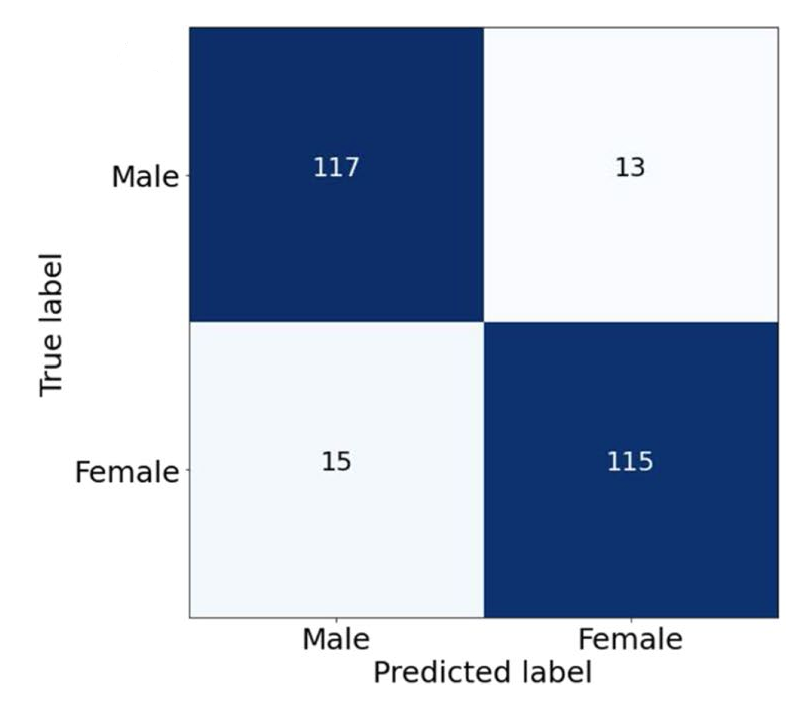
\includegraphics[width=0.6\textwidth]{capitulos/cap_02/imagenes/confusion_matrix_binary.png}
        \caption{
            Matriz de confusión para la estimación de sexo según el modelo \textit{random forest} propuesto en \cite{bidmos2023}.
        } 
        \label{fig:conf_matrix_binary}
    \end{figure}
    
    % \begin{figure}[h]
    %     \centering
    
    %     \begin{subfigure}[b]{0.3\textwidth}
    %         \centering
    %         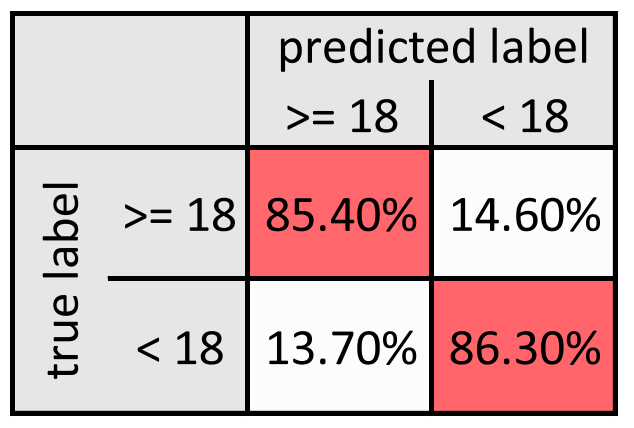
\includegraphics[width=\textwidth]{capitulos/cap_02/imagenes/confusion_matrix_binary_1.png}
    %         \caption{Sin información de sexo}
    %         \label{fig:conf_matrix_general}
    %     \end{subfigure}
    %     \hfill
    %     \begin{subfigure}[b]{0.3\textwidth}
    %         \centering
    %         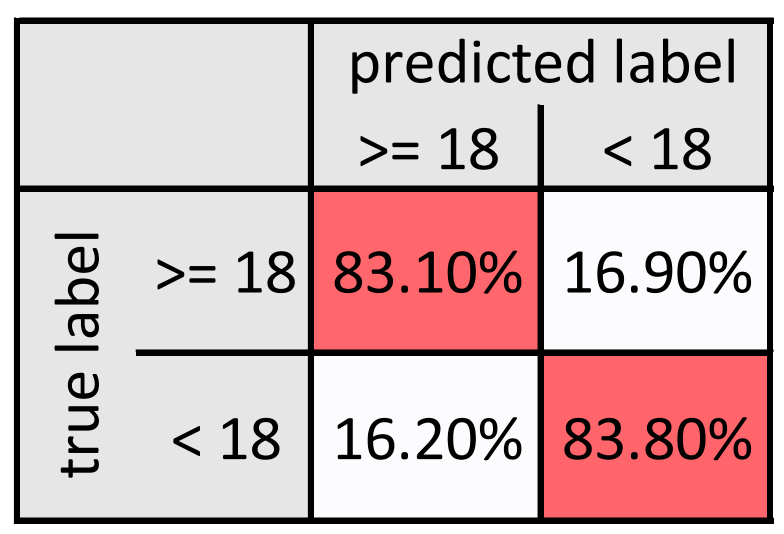
\includegraphics[width=\textwidth]{capitulos/cap_02/imagenes/confusion_matrix_binary_2.png}
    %         \caption{Sexo femenino}
    %         \label{fig:conf_matrix_female}
    %     \end{subfigure}
    %     \hfill
    %     \begin{subfigure}[b]{0.3\textwidth}
    %         \centering
    %         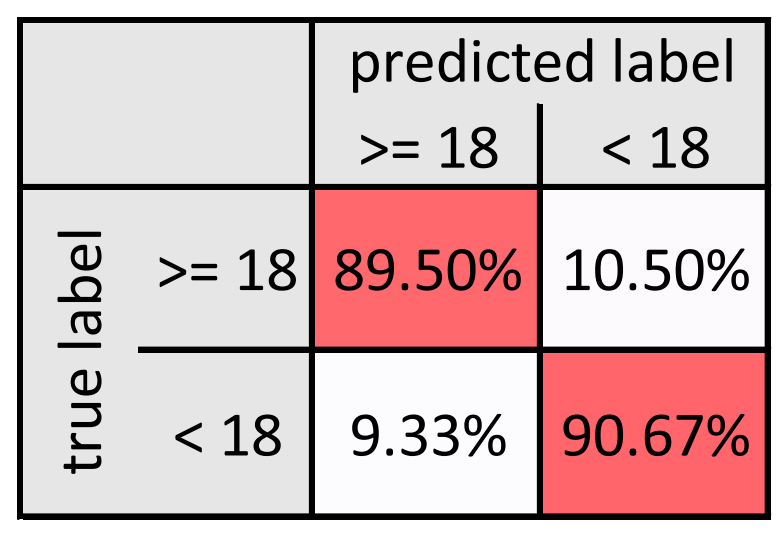
\includegraphics[width=\textwidth]{capitulos/cap_02/imagenes/confusion_matrix_binary_3.png}
    %         \caption{Sexo masculino}
    %         \label{fig:conf_matrix_male}
    %     \end{subfigure}
    
    %     \caption[
    %         Matrices de confusión para la estimación de mayoría/minoría de edad según el modelo de 
    %         \cite{porto2020}.
    %     ]{
    %         Matrices de confusión para la estimación de mayoría/minoría de edad según el modelo de 
    %         \cite{porto2020}.
    %         Se representan los valores de cada celda en términos porcentuales de los ejemplos reales que hay 
    %         de cada clase ($< 18$ y $\ge 18$), lo que permite comparar la matriz de confusión general de todos 
    %         los ejemplos (\ref{sub@fig:conf_matrix_general}) con la de ejemplos se sexo femenino 
    %         (\ref{sub@fig:conf_matrix_female}) y sexo masculino (\ref{sub@fig:conf_matrix_male}), permitiendo 
    %         identificar posibles sesgos en el modelo respecto al género, y así realizar una evaluación más 
    %         precisa del rendimiento del modelo en diferentes subgrupos de la población.
    %     }
    %     \label{fig:conf_matrix_binary_relative}

    % \end{figure}


    \item La \textbf{cobertura empírica (\textit{empirical coverage})}, de forma análoga a la regresión, mide la proporción de veces que la etiqueta verdadera está contenida dentro del conjunto predicho.

    $$
    EC = \frac{1}{n} \sum_{i=1}^{n} \mathbb{I}(y_i \in \Gamma_\alpha(x_i))
    $$

    \item El \textbf{tamaño medio del conjunto de predicción (\textit{mean prediction set size})} mide qué cuántas etiquetas, en promedio, incluyen los conjuntos de predicción $\Gamma_\alpha(x)$.

    $$
    MSS = \frac{1}{n} \sum_{i=1}^n | \Gamma_\alpha(x_i) |
    $$

\end{itemize}


% ------------------------------------------------------------------------------------------------------------
% ------------------------------------------------------------------------------------------------------------

\section{Resultados}

% ------------------------------------------------------------------------------------------------------------

\subsection{Resultados para la estimación de edad}

\subsubsection{Análisis de métricas para la estimación de edad puntual}

La Tabla \ref{tab:AE_MAE_MSE_comparative} presenta las métricas que evalúan el rendimiento del modelo de regresión en sus estimaciones del valor esperado de edad. En general, se observa \textbf{poca variabilidad entre modelos y ejecuciones}, con diferencias de solo unas centésimas en las métricas evaluadas. Sin embargo, el análisis de varianza (ANOVA)%
\footnote{
    La aplicación del ANOVA se basó en las suposiciones de independencia entre errores medios por modelo y ejecución, normalidad aproximada de los residuos y homogeneidad de varianzas entre grupos.
} 
de un factor reveló diferencias estadísticamente significativas entre los modelos para ambas métricas: MAE ($F(3, 28) = 20.38$, $p < 0.001$) y MSE ($F(3, 28) = 15.09$, $p < 0.001$). Para identificar qué pares de modelos presentaban diferencias significativas, se aplicó la prueba \textit{post-hoc} de comparaciones múltiples de Tukey (véanse las Tablas \ref{tab:AE_tukey_mae} y \ref{tab:AE_tukey_mse}). Los resultados indicaron lo siguiente:

\todo{¿Debería indicar los supuestos a la hora de usar ANOVA y Tukey? Por ejemplo: se asume que cada método presenta distribución normal en las métricas}

\renewcommand{\arraystretch}{1.4}
\begin{table}[h]
    \small
    \begin{tabular}{clcccclcccc}
    % \hline
    \toprule
    \multirow{2}{*}{\textbf{Método}} &  & \multicolumn{4}{c}{\textbf{Error Absoluto Medio}}         &  & \multicolumn{4}{c}{\textbf{Error Cuadrático Medio}}           \\ \cline{3-6} \cline{8-11} 
                                    &  & \textbf{base} & \textbf{ICP} & \textbf{QR} & \textbf{CQR}  &  & \textbf{base} & \textbf{ICP} & \textbf{QR} & \textbf{CQR} \\ \cline{1-1} \cline{3-6} \cline{8-11} 
    Ejecución 1                      &  & 1.17          & 1.20         & 1.17        & 1.18         &  & 2.39          & 2.50         & 2.38        & 2.46         \\
    Ejecución 2                      &  & 1.15          & 1.18         & 1.17        & 1.20         &  & 2.33          & 2.45         & 2.40        & 2.49         \\
    Ejecución 3                      &  & 1.17          & 1.21         & 1.17        & 1.17         &  & 2.38          & 2.55         & 2.42        & 2.36         \\
    Ejecución 4                      &  & 1.16          & 1.20         & 1.14        & 1.17         &  & 2.34          & 2.47         & 2.32        & 2.41         \\
    Ejecución 5                      &  & 1.16          & 1.21         & 1.16        & 1.18         &  & 2.37          & 2.52         & 2.39        & 2.42         \\
    Ejecución 6                      &  & 1.15          & 1.20         & 1.17        & 1.17         &  & 2.33          & 2.51         & 2.40        & 2.40         \\
    Ejecución 7                      &  & 1.16          & 1.20         & 1.18        & 1.19         &  & 2.34          & 2.48         & 2.46        & 2.43         \\
    Ejecución 8                      &  & 1.18          & 1.20         & 1.17        & 1.20         &  & 2.39          & 2.43         & 2.40        & 2.47         \\
    Ejecución 9                      &  &               &              &             &              &  &               &              &             &              \\
    Ejecución 10                     &  &               &              &             &              &  &               &              &             &              \\ \cline{1-1} \cline{3-6} \cline{8-11} 
    Media                            &  & 1.16          & 1.20         & 1.16        & 1.19         &  & 2.36          & 2.49         & 2.38        & 2.44         \\ 
    \bottomrule
    \end{tabular}
    \caption[
        Error absoluto medio y error cuadrático medio obtenidos por cada método de predicción a lo largo de distintas ejecuciones.
    ]{
        Error absoluto medio y error cuadrático medio obtenidos por cada método de predicción a lo largo de distintas ejecuciones. 
        Se presentan los valores para cada ejecución individual, así como la media final de cada métrica. Punto como separador decimal.
    }
    \label{tab:AE_MAE_MSE_comparative}
\end{table}

\renewcommand{\arraystretch}{1.2}
\begin{table}[h]
    \small
    \centering
    \begin{tabular}{llllll}
    \toprule
    \textbf{Modelo 1} & \textbf{Modelo 2} & \textbf{Dif. media} & \textbf{Valor $p$} & \textbf{IC 95\%} & \textbf{Signif.} \\
    \midrule
    CQR  & ICP   & 0.0122 & 0.176  & [-0.0036,\ 0.0279] & No  \\
    CQR  & QR    & -0.0244 & 0.0013 & [-0.0401,\ -0.0086] & \textbf{Sí} \\
    CQR  & base  & -0.0250 & 0.0010 & [-0.0407,\ -0.0092] & \textbf{Sí} \\
    ICP  & QR    & -0.0365 & \textless 0.0001 & [-0.0523,\ -0.0208] & \textbf{Sí} \\
    ICP  & base  & -0.0371 & \textless 0.0001 & [-0.0529,\ -0.0214] & \textbf{Sí} \\
    QR   & base  & -0.0006 & 0.9996 & [-0.0164,\ 0.0152] & No \\
    \bottomrule
    \end{tabular}
    \caption[
        Resultados de la prueba \textit{post-hoc} de Tukey HSD para MAE entre pares de modelos.
    ]{
        Resultados de la prueba \textit{post-hoc} de Tukey HSD para MAE entre pares de modelos. 
        Se muestran la diferencia media entre grupos, el valor $p$ ajustado, el intervalo de confianza al 95\% y si la diferencia es estadísticamente significativa ($\alpha = 0.05$).
    }
    \label{tab:AE_tukey_mae}
\end{table}

\renewcommand{\arraystretch}{1.2}
\begin{table}[h]
    \small
    \centering
    \begin{tabular}{llllll}
    \toprule
    \textbf{Modelo 1} & \textbf{Modelo 2} & \textbf{Dif. media} & \textbf{Valor $p$} & \textbf{IC 95\%} & \textbf{Signif.} \\
    \midrule
    CQR  & ICP   & 0.0484  & 0.1353   & [-0.0104,\ 0.1072]     & No            \\
    CQR  & QR    & -0.0595 & 0.0464   & [-0.1183,\ -0.0007]    & \textbf{Sí}   \\
    CQR  & base  & -0.0825 & 0.0035   & [-0.1413,\ -0.0237]    & \textbf{Sí}   \\
    ICP  & QR    & -0.1079 & 0.0002   & [-0.1667,\ -0.0491]    & \textbf{Sí}   \\
    ICP  & base  & -0.1309 & \textless 0.0001  & [-0.1896,\ -0.0721]    & \textbf{Sí}   \\
    QR   & base  & -0.0229 & 0.7128   & [-0.0817,\ 0.0358]     & No            \\
    \bottomrule
    \end{tabular}
    \caption[
        Resultados de la prueba \textit{post-hoc} de Tukey HSD para MSE entre pares de modelos.
    ]{
        Resultados de la prueba \textit{post-hoc} de Tukey HSD para MSE entre pares de modelos. 
        Se muestran la diferencia media entre grupos, el valor $p$ ajustado, el intervalo de confianza al 95\% y si la diferencia es estadísticamente significativa ($\alpha = 0.05$).
    }
    \label{tab:AE_tukey_mse}
\end{table}

\begin{itemize}
    
    \item No se encontraron diferencias significativas entre los modelos `QR' y `base' en ninguna métrica, al igual que tampoco entre los modelos `CQR' e `ICP', lo que sugiere rendimientos similares entre estos pares de modelos. Esto indica que los modelos de regresión cuantílica obtiene resultados equivalentes a los modelos de regresión central.  

    \item Los modelos conformales (`ICP' y `CQR') mostraron errores significativamente mayores ($p<0.01$) que los modeloss no conformales (`base' y `QR'). Esto era esperable, pues los métodos conformales tienen menos ejemplos para entrenarse y, por tanto, generalizan peor. 

\end{itemize}


\subsubsection{Análisis de métricas para la estimación de edad interválica}

A continuación, la Tabla \ref{tab:AE_EC_MPIW_comparative} presenta las métricas sobre las predicciones interválicas de los métodos. A primera vista, se observan diferencias marcadas entre los métodos conformales y no conformales en las métricas de cobertura empírica y amplitud del intervalo. En particular, los métodos no conformales (`base' y QR) muestran coberturas inferiores al nivel deseado (alrededor del 88-89\% frente al 95\% nominal), lo que indica una infracobertura sistemática. Esto ocurre porque ni la heurística del método `base' ni las regiones generadas por la regresión cuantílica en QR cuentan con garantías teóricas de cobertura estadística.

\renewcommand{\arraystretch}{1.5}
\begin{table}[h]
    \small 
    \centering
    \begin{tabular}{cc@{\hskip 3pt}ccccc@{\hskip 3pt}cccc}
    \toprule
    \multirow{2}{*}{\textbf{Método}} &  & \multicolumn{4}{c}{\textbf{Cobertura Empírica (\%)}}      &  & \multicolumn{4}{c}{\textbf{\begin{tabular}[c]{@{}c@{}}Amplitud Media \\[-0.8ex] del Intervalo\end{tabular}}}          \\ \cline{3-6} \cline{8-11} 
                                     &  & \textbf{base} & \textbf{ICP} & \textbf{QR} & \textbf{CQR} &  & \textbf{base} & \textbf{ICP} & \textbf{QR} & \textbf{CQR} \\ \cline{1-1} \cline{3-6} \cline{8-11} 
    Ejecución 1                      &  & 87.41         & 94.47        & 89.03       & 95.31        &  & 4.53          & 6.17         & 4.71        & 6.23         \\
    Ejecución 2                      &  & 87.96         & 94.84        & 89.27       & 94.8         &  & 4.57          & 6.27         & 4.67        & 6.11         \\
    Ejecución 3                      &  & 87.73         & 95.03        & 88.38       & 95.45        &  & 4.60          & 6.34         & 4.65        & 6.02         \\
    Ejecución 4                      &  & 88.06         & 94.19        & 89.5        & 94.61        &  & 4.58          & 6.04         & 4.63        & 5.90         \\
    Ejecución 5                      &  & 87.87         & 95.03        & 89.13       & 94.93        &  & 4.63          & 6.28         & 4.59        & 5.92         \\
    Ejecución 6                      &  & 88.62         & 95.91        & 89.73       & 95.17        &  & 4.71          & 6.52         & 4.66        & 5.98         \\
    Ejecución 7                      &  & 88.24         & 95.21        & 88.8        & 95.26        &  & 4.61          & 6.33         & 4.63        & 6.00         \\
    Ejecución 8                      &  & 87.55         & 94.7         & 88.01       & 95.12        &  & 4.64          & 6.12         & 4.67        & 6.08         \\
    Ejecución 9                      &  &               &              &             &              &  &               &              &             &              \\
    Ejecución 10                     &  &               &              &             &              &  &               &              &             &              \\ \cline{1-1} \cline{3-6} \cline{8-11} 
    Media                            &  & 87.93         & 94.92        & 88.98       & 95.08        &  & 4.61          & 6.26         & 4.65        & 6.03         \\ 
    \bottomrule
    \end{tabular}
    \caption[
        Cobertura empírica y amplitud media del intervalo de predicción obtenidos por cada método de predicción a lo largo de distintas ejecuciones.
    ]{   
        Cobertura empírica y amplitud media del intervalo de predicción obtenidos por cada método de predicción a lo largo de distintas ejecuciones. 
        Se presentan los valores para cada ejecución individual, así como la media final de cada métrica. Punto como separador decimal.
    }
    \label{tab:AE_EC_MPIW_comparative}
\end{table}

En contraste, los métodos conformales (ICP y CQR) sí logran coberturas próximas al valor nominal, tal como se espera dada su fundamentación estadística. Esta mayor cobertura, sin embargo, tiene un costo en cuanto a la amplitud del intervalo, que tiende a ser mayor que en los métodos conformales. Esta relación de compromiso o \textit{trade-off} entre cobertura y amplitud de los intervalos ---típico en la predicción interválica--- se visualiza claramente en la Figura \ref{fig:AE_scatterplot_EC-MPIW}, donde se observa una alta correlación entre la cobertura empírica y el tamaño del intervalo de predicción.

\begin{figure}[h]
    \centering
    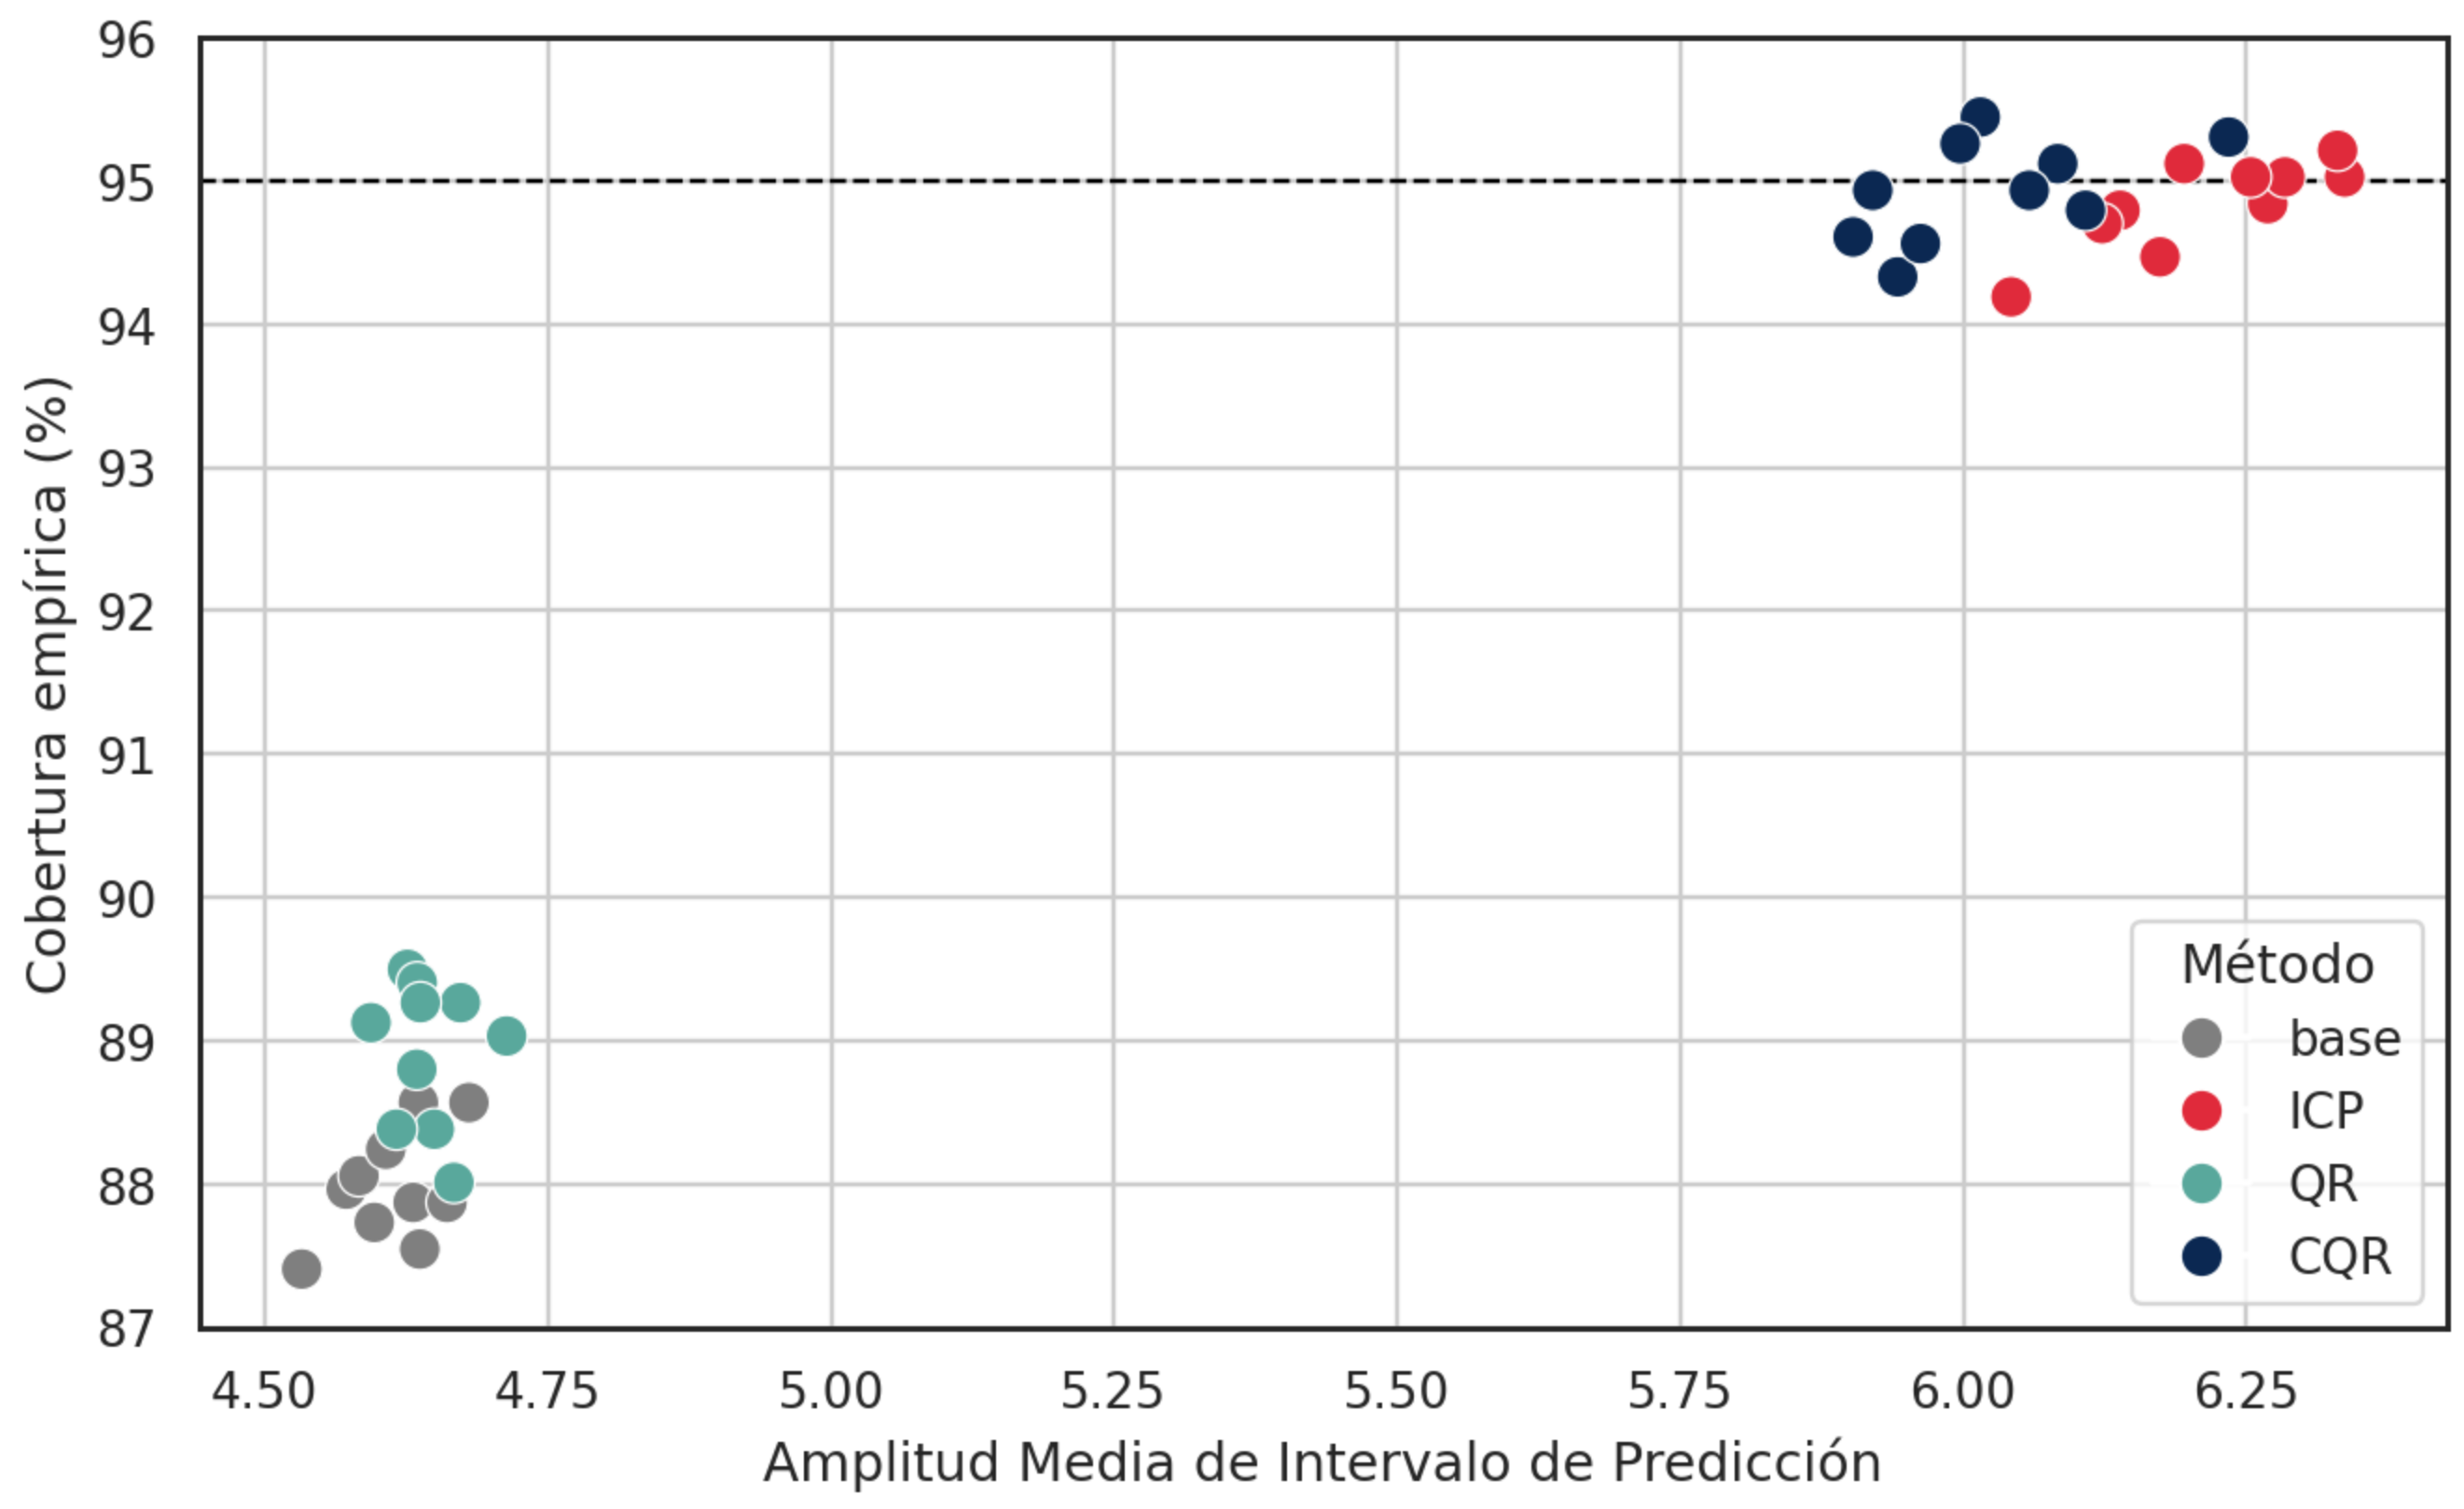
\includegraphics[width=\textwidth]{capitulos/cap_05/imagenes/AE_scatterplot_EC-MPIW.png}
    \caption[
        Gráfica de dispersión \textit{Empirical Coverage}-\textit{Mean Precition Interval Width}
    ]{
        Gráfica de dispersión \textit{Empirical Coverage}-\textit{Mean Precition Interval Width}. 
    }
    \label{fig:AE_scatterplot_EC-MPIW}
\end{figure}

Sin embargo, CQR presenta unas amplitudes promedias de intervalo significativamente más reducidas que ICP, logrando ambos métodos coberturas muy similares. De hecho, en la Tabla \ref{tab:AE_MIS_comparative} apreciamos cómo CQR logra significativamente menores valores de \textit{interval score} que ICP, indicando que CQR tiene un mejor equilibrio entre cobertura y tamaño del intervalo.

En consecuencia, CQR se perfila como una opción más ventajosa, con garantías de cobertura e intervalos de predicción ajustados. 

\todo{Apliqué ANOVA y Tukey aquí, pero no resultaron muy útiles ya que no tienen en cuenta la relación de correlación entre cobertura empírica y tamaño medio del intervalo, y resultaba en que ICP y CQR no mostraban coberturas significativamente diferentes, lo que es verdad, pero no presenta una información completa. ¿Merece la pena hacer MANOVA (ANOVA para múltiples variables) o directamente con la figura ya queda claro?}

\renewcommand{\arraystretch}{1.5}
\begin{table}[h]
    \small \centering
    \begin{tabular}{cccccc}
    \toprule
    \multirow{2}{*}{\textbf{Método}} &  & \multicolumn{4}{c}{\textbf{Mean Interval Score}}          \\ \cline{3-6} 
                                     &  & \textbf{base}  & \textbf{ICP}  & \textbf{QR}   & \textbf{CQR} \\ \cline{1-1} \cline{3-6} 
    Ejecución 1                      &  & 9.16           & 8.17          & 8.48          & 8.02         \\
    Ejecución 2                      &  & 8.93           & 8.21          & 8.72          & 8.04         \\
    Ejecución 3                      &  & 8.90           & 8.24          & 8.86          & 7.85         \\
    Ejecución 4                      &  & 8.69           & 8.00          & 8.59          & 7.98         \\
    Ejecución 5                      &  & 8.88           & 8.27          & 8.82          & 7.89         \\
    Ejecución 6                      &  & 8.75           & 8.23          & 8.40          & 8.06         \\
    Ejecución 7                      &  & 8.81           & 8.19          & 8.96          & 7.85         \\
    Ejecución 8                      &  & 8.88           & 8.03          & 8.8           & 7.91         \\
    Ejecución 9                      &  &                &               &               &              \\
    Ejecución 10                     &  &                &               &               &              \\ \cline{1-1} \cline{3-6} 
    Media                            &  & 8.88           & 8.17          & 8.71          & 7.95         \\ 
    \bottomrule
    \end{tabular}
    \caption[
        Resultados de las predicciones obtenidas por los modelos para el problema de estimación de edad en cada ejecución.
    ]{   
        Resultados de las predicciones obtenidas por los modelos para el problema de estimación de edad en cada ejecución.
        Punto como separador decimal.
    }
    \label{tab:AE_MIS_comparative}
\end{table}

\FloatBarrier

\subsubsection{Análisis de la cobertura en base al tamaño del intervalo}

En los métodos donde los intervalos de predicción varían en amplitud entre instancias (QR y CQR), resulta relevante analizar cómo se comporta la cobertura empírica en función de dicho tamaño. La hipótesis subyacente es que intervalos más amplios reflejan una mayor incertidumbre asociada a la predicción, mientras que intervalos más estrechos denotan mayor confianza.

Particularmente, se busca determinar si los intervalos más estrechos tienden a infracubrir (es decir, no contienen el valor real con la frecuencia esperada), y si los intervalos más amplios tienden a sobrecubrir (conteniendo el valor real más allá del nivel objetivo de confianza).

En la Figura \ref{fig:AE_EC_by_PIW} se presentan los histogramas de la amplitud de los intervalos de predicción para dos modelos representativos, uno QR y otro CQR. En cada caso, se diferencia visualmente la proporción de instancias cuya predicción cubre el valor real de aquellas en las que no lo hace. Es notable en ambas figuras la presencia de dos grupos principales de instancias: uno más reducido, asociado a intervalos más estrechos, y otro más numeroso, correspondiente a intervalos de mayor amplitud. Respecto a la cobertura, el modelo QR presenta valores inferiores, lo cual es consistente con su cobertura marginal, que ya se encontraba por debajo del 89\%. En cuanto al ratio entre cobertura e incobertura, este parece mantenerse relativamente estable a lo largo de los distintos rangos de amplitud del intervalo. Sin embargo, para un análisis más detallado y específico sobre cómo varía la cobertura en función del tamaño del intervalo, observemos la información desglosada en la Tabla \ref{tab:AE_EC_by_PIW}.

\todo{Esto ocurre, pero no sé por qué. Voy a investigar, pero me temo que va a ser difícil hallar la razón, ya que muy probablemente sea fruto del funcionamiento de la red en regresión cuantílica, y al ser un modelo de caja negra, no pueda hacer nada.}

\begin{figure}[h]
    \centering

    \begin{subfigure}[b]{0.8\textwidth}
        \centering
        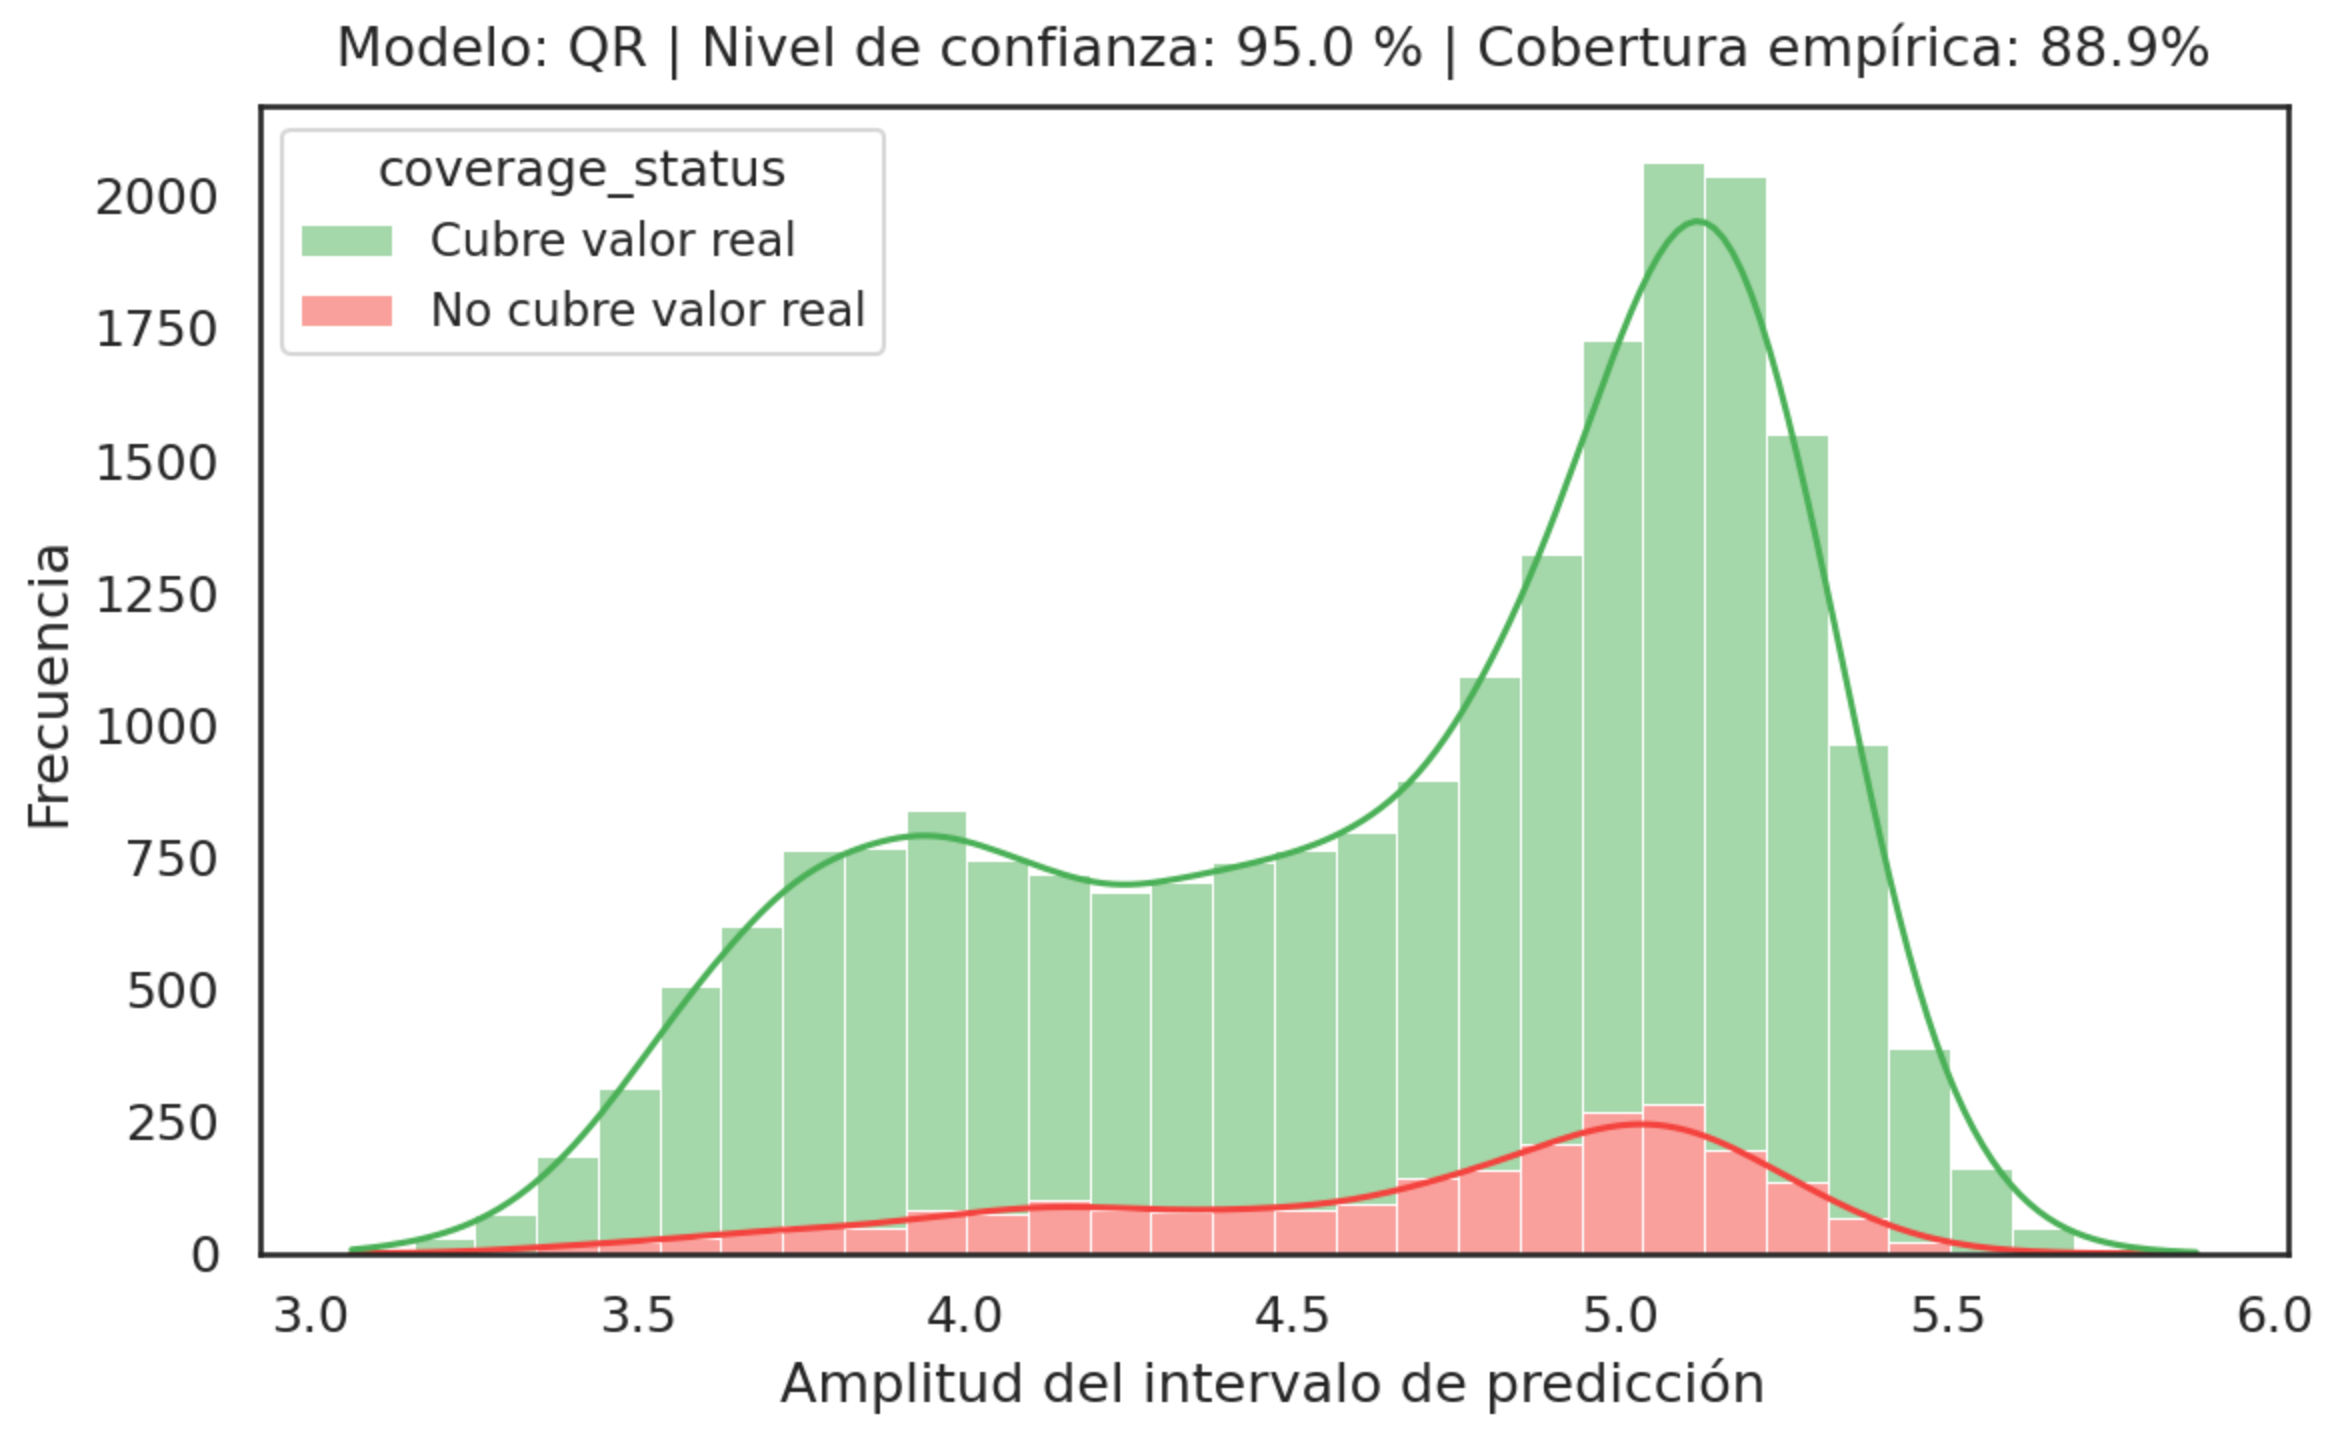
\includegraphics[width=\textwidth]{capitulos/cap_05/imagenes/AE_histogram_EC_by_PIW_QR.png}
        \caption{
            Histograma de amplitud del intervalo de predicción con diferenciación por cobertura (modelo QR).
        }
        \label{fig:AE_EC_by_PIW_QR}
    \end{subfigure}

    \vspace{0.5cm}
    
    \begin{subfigure}[b]{0.8\textwidth}
        \centering
        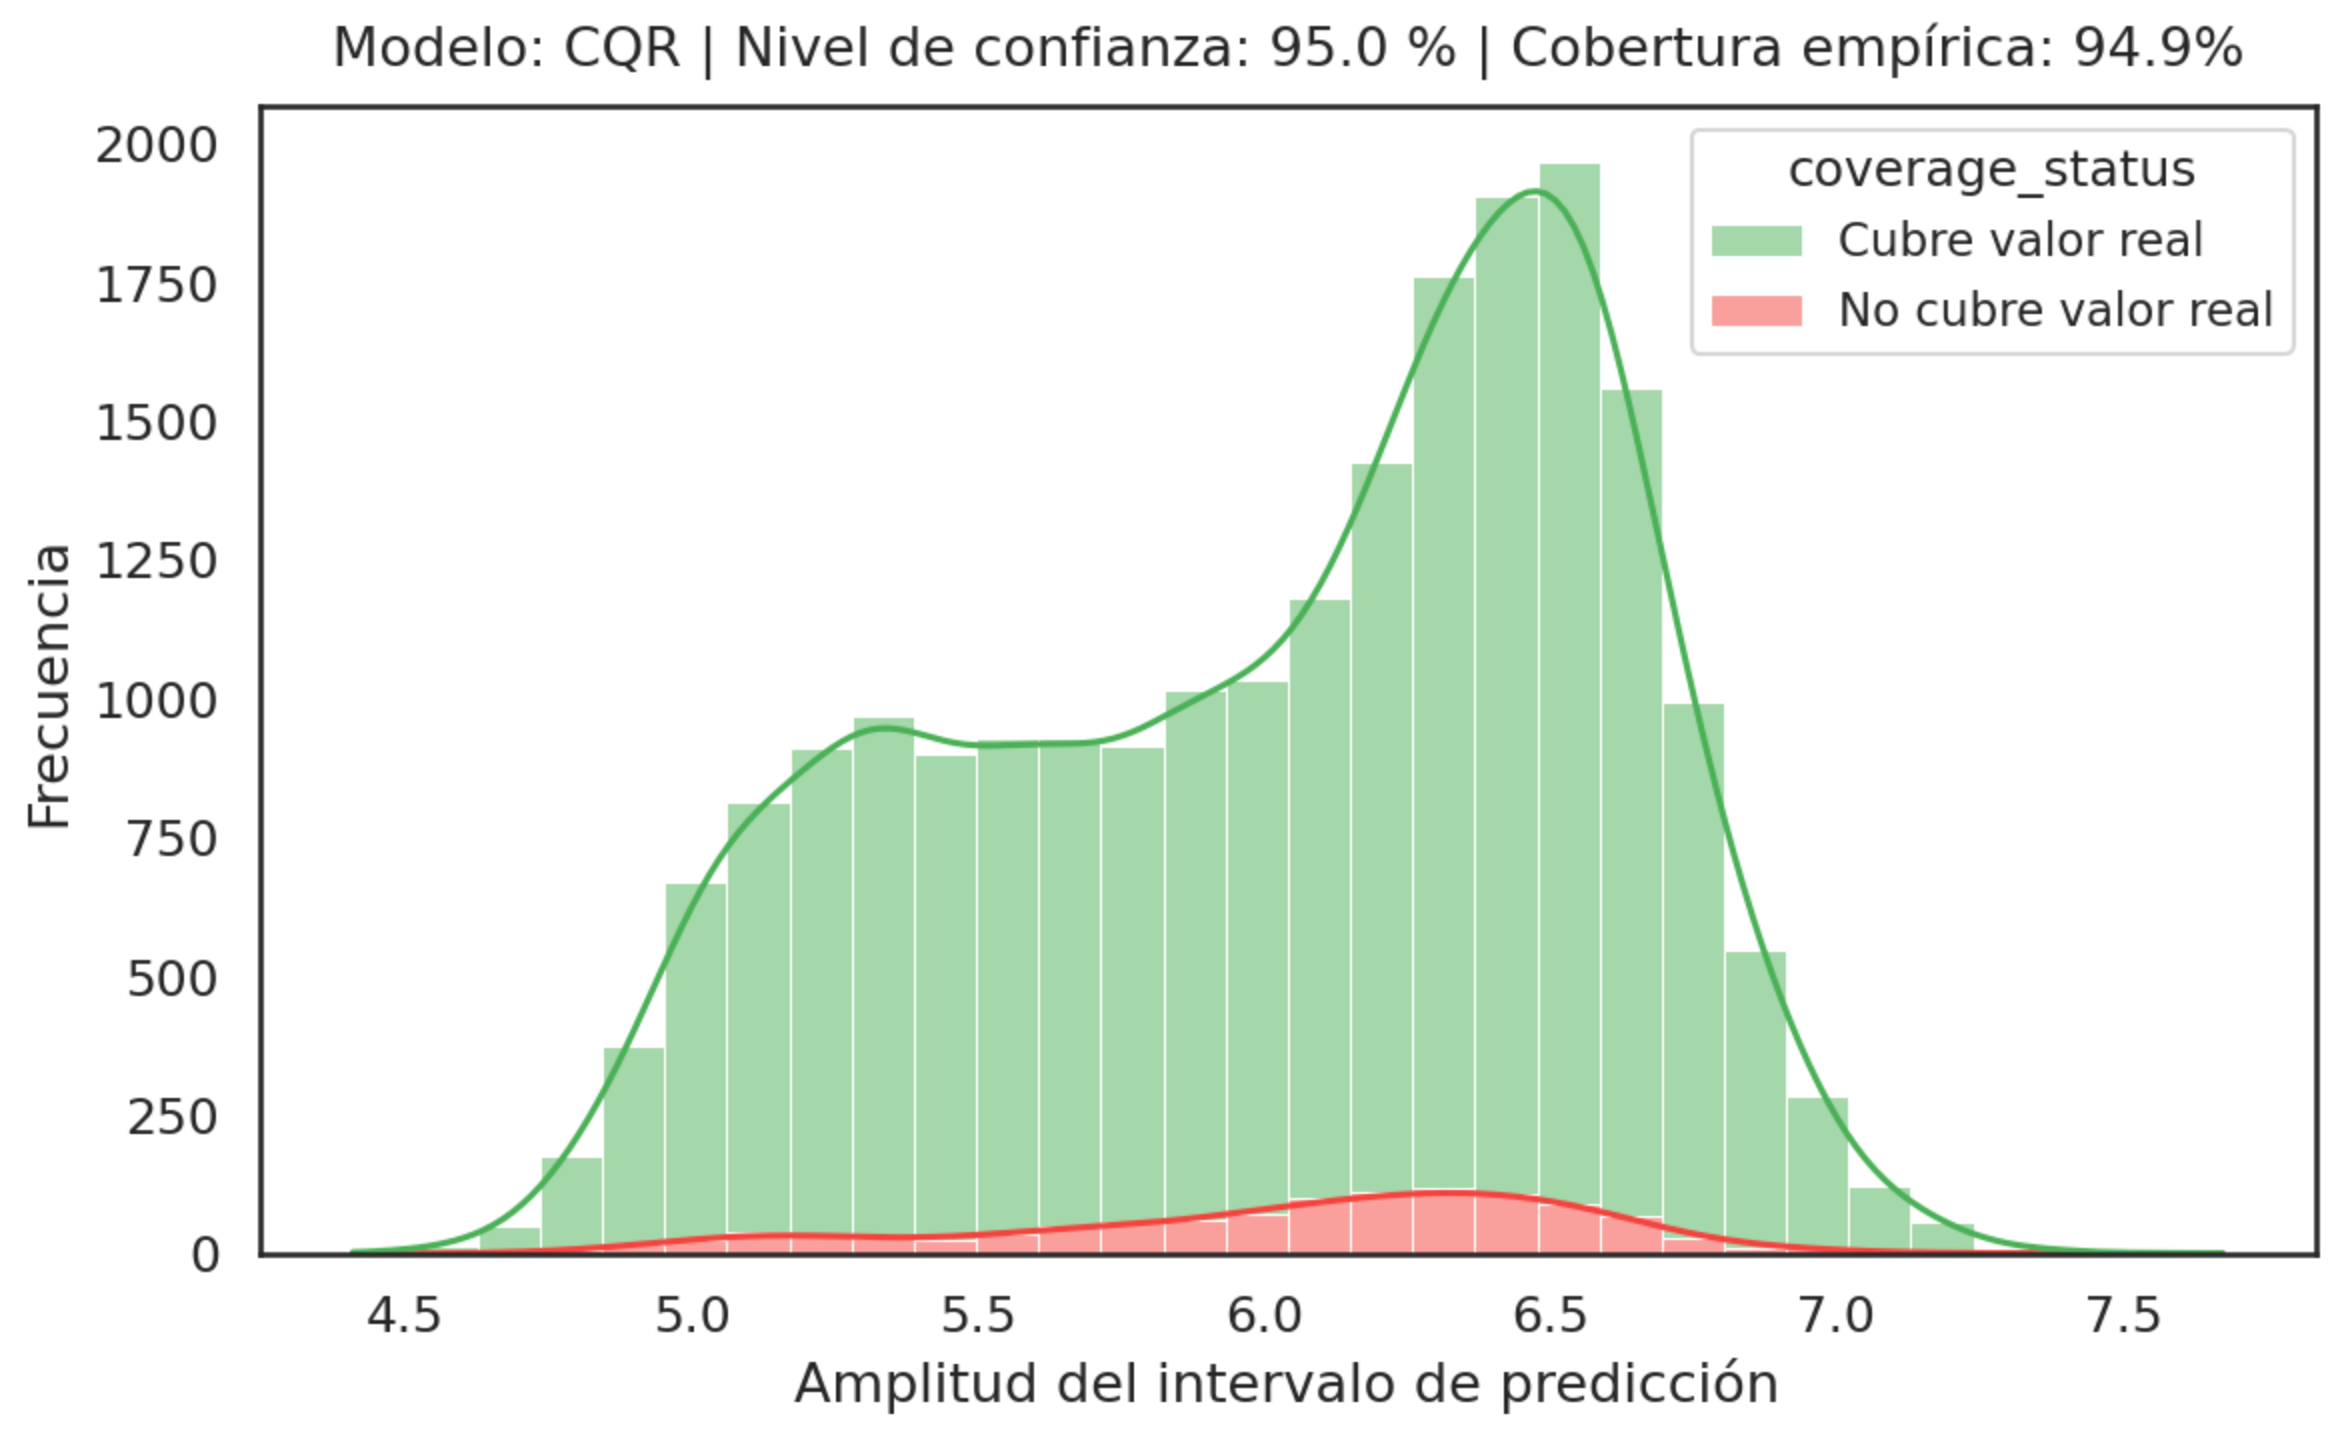
\includegraphics[width=\textwidth]{capitulos/cap_05/imagenes/AE_histogram_EC_by_PIW_CQR.png}
        \caption{
            Histograma de amplitud del intervalo de predicción con diferenciación por cobertura (modelo CQR).
        }
        \label{fig:AE_EC_by_PIW_CQR}
    \end{subfigure}

    \caption[
        Histogramas del amplitud del intervalo de predicción con diferenciación por cobertura, correspondientes a los modelos QR y CQR.
    ]{
        Histogramas del amplitud del intervalo de predicción con diferenciación por cobertura, correspondientes a los modelos QR y CQR. 
        Para cada tipo de método se seleccionó el modelo con el mejor \textit{interval score}. La comparación permite visualizar cómo varía la capacidad de cobertura en función del tamaño del intervalo.
    }
    \label{fig:AE_EC_by_PIW}
\end{figure}

En la Tabla \ref{tab:AE_EC_by_PIW} se ofrece información detallada sobre la cobertura empírica alcanzada por cada método de predicción (en todas sus ejecuciones) en función de diferentes rangos de amplitud del intervalo de predicción. Esta desagregación permite analizar si existe una relación entre el tamaño del intervalo y la capacidad del modelo para cubrir el valor real. 

Como era de esperar, los modelos basados en regresión cuantílica (QR y CQR) presentan una mayor diversidad en la amplitud de sus intervalos, dado que generan límites adaptativos y específicos para cada instancia, a diferencia de los métodos conformales de tamaño más constante.

Llama la atención que se logra sobrecobertura tanto en los intervalos más estrechos como en los más amplios, a costa de una infracobertura en los intervalos de amplitud intermedia, concretamente entre 5.5 y 6.5 años, siendo especialmente más bajas en el último medio tramo, donde la cobertura alcanza un 93.4\%.

\todo{No estoy entrando a hacer valoraciones de lo grave o leve que sea que la cobertura se reduzca de un 95 a un 93.4, porque entiendo que aquí entraría mi subjetividad, y esa debe ir más en las conclusiones que aquí, ¿correcto?}

\renewcommand{\arraystretch}{1.4}
\begin{table}[h]
    \centering
    \begin{tabular}{cccccccc}
        \toprule
        \multicolumn{2}{c}{\multirow{2}{*}{\textbf{Método}}} & & \multicolumn{4}{c}{\textbf{Cobertura Empírica (\%)}} \\ \cmidrule{4-7}
        \multicolumn{2}{c}{} & & \textbf{base} & \textbf{ICP} & \textbf{QR} & \textbf{CQR} \\ \midrule
        \multirow{8}{*}{\begin{tabular}[c]{@{}c@{}}Amplitud del\\ intervalo\end{tabular}} 
        & $[4.0 , 4.5)$  & & --    & --    & 91.58 & 100   \\
        & $[4.5 , 5.0)$  & & 87.93 & --    & 92.85 & 96.32 \\
        & $[5.0 , 5.5)$  & & --    & --    & 88.45 & 96.47 \\
        & $[5.5 , 6.0)$  & & --    & --    & 85.62 & 94.82 \\
        & $[6.0 , 6.5)$  & & --    & 94.78 & 89.43 & 93.40 \\
        & $[6.5 , 7.0)$  & & --    & 95.91 & 97.14 & 96.09 \\
        & $[7.0 , 7.5)$  & & --    & --    & --    & 97.37 \\
        & $[7.5 , 8.0)$  & & --    & --    & --    & 100   \\
        \bottomrule
    \end{tabular}
    \caption[
        Cobertura empírica del intervalo de predicción obtenida por cada método de predicción para distintas franjas de amplitud de intervalos.
    ]{
        Cobertura empírica del intervalo de predicción obtenida por cada método de predicción para distintas franjas de amplitud de intervalos. Nota: Los métodos de intervalos de tamaño fijo (como ICP, en este caso) pueden mostrar varias franjas debido a que los tamaños de intervalo pueden variar ligeramente entre entrenamientos para un mismo método.     
    }
    \label{tab:AE_EC_by_PIW}
\end{table}

\FloatBarrier


\subsubsection{Análisis de la cobertura en base a la edad cronológica}

Por último, se ha analizado la cobertura en base a la edad real de los individuos. En la Tabla \ref{tab:AE_EC_by_true_age} se presentan las métricas interválicas para las instancias de cada edad cronológica%
\footnote{
    Parte entera (suelo) de la edad real.
}.
La Figura \ref{fig:AE_EC_MPIW_by_true_age} muestra la evolución de la cobertura empírica y el ancho medio de los intervalos de predicción en función de la edad.

Se observa que todos los métodos tienden a reducir su cobertura conforme aumenta la edad cronológica de los individuos. Esta disminución es especialmente notable a partir de los 22 años, afectando incluso al método CQR, que es el método con la cobertura más robusta.

En particular, CQR logra mantener una cobertura cercana al 95\% para individuos de hasta 22 años, pero a partir de los 23 comienza a descender, alcanzando aproximadamente un 85\% en los individuos de 25 años. Este descenso ocurre a pesar de que el tamaño de los intervalos de predicción aumenta de forma sostenida con la edad, lo que indica que, aunque el modelo expresa mayor incertidumbre, no consigue cubrir adecuadamente el valor real. Este patrón refleja que la estimación de la edad biológica se vuelve más incierta conforme avanza la edad cronológica, posiblemente debido a una mayor heterogeneidad fisiológica, ya que este grupo estaba igualmente representado que el resto de edades en el conjunto de entrenamiento.

\todo{¿Esto último debería ir en las conclusiones?}

\renewcommand{\arraystretch}{1.5}
\begin{table}[]
    \small
    \centering
    \begin{tabular}{cccccccccccc}
    \toprule
    \multirow{2}{*}{\textbf{Método}} &  & \multicolumn{4}{c}{\textbf{Cobertura Empírica (\%)}}      &  & \multicolumn{4}{c}{\textbf{\begin{tabular}[c]{@{}c@{}}Amplitud Media \\[-0.8ex] del Intervalo\end{tabular}}} \\ \cline{3-6} \cline{8-11} 
                                    &  & \textbf{base} & \textbf{ICP} & \textbf{QR} & \textbf{CQR} &  & \textbf{base}            & \textbf{ICP}            & \textbf{QR}           & \textbf{CQR}           \\ \cline{1-1} \cline{3-6} \cline{8-11} 
    Edad 14                          &  & 92.82         & 97.52        & 91.27       & 96.1         &  & 4.61                     & 6.26                    & 3.74                  & 5.15                   \\
    Edad 15                          &  & 88.92         & 96.05        & 90.09       & 95.22        &  & 4.61                     & 6.26                    & 3.98                  & 5.37                   \\
    Edad 16                          &  & 90.33         & 95.43        & 91.58       & 95.27        &  & 4.61                     & 6.26                    & 4.23                  & 5.61                   \\
    Edad 17                          &  & 89.77         & 96.11        & 90.31       & 95.28        &  & 4.61                     & 6.26                    & 4.46                  & 5.82                   \\
    Edad 18                          &  & 85.74         & 95.45        & 86.65       & 95.21        &  & 4.61                     & 6.26                    & 4.65                  & 6                      \\
    Edad 19                          &  & 90.1          & 97.07        & 91.26       & 96.79        &  & 4.61                     & 6.26                    & 4.87                  & 6.22                   \\
    Edad 20                          &  & 90.88         & 97.04        & 93.72       & 97.52        &  & 4.61                     & 6.26                    & 4.99                  & 6.36                   \\
    Edad 21                          &  & 92.4          & 97.24        & 93.75       & 97.12        &  & 4.61                     & 6.26                    & 5.09                  & 6.47                   \\
    Edad 22                          &  & 86.9          & 94.01        & 87.2        & 94.39        &  & 4.61                     & 6.26                    & 5.14                  & 6.51                   \\
    Edad 23                          &  & 79.17         & 90.1         & 81.55       & 92.04        &  & 4.61                     & 6.26                    & 5.2                   & 6.6                    \\
    Edad 24                          &  & 74.54         & 83.49        & 75.31       & 87.04        &  & 4.61                     & 6.26                    & 5.29                  & 6.7                    \\
    Edad 25                          &  & 63.75         & 76.25        & 66.25       & 85.62        &  & 4.61                     & 6.26                    & 5.37                  & 6.8                    \\ 
    \bottomrule
    \end{tabular}
    \caption[
        Cobertura empírica y amplitud media del intervalo de predicción obtenidos por cada método de predicción para distintas edades cronológicas.
    ]{
        Cobertura empírica y amplitud media del intervalo de predicción obtenidos por cada método de predicción para distintas edades cronológicas.
    }
    \label{tab:AE_EC_by_true_age}
\end{table}




\begin{figure}[h]
    \centering

    \begin{subfigure}[b]{0.9\textwidth}
        \centering
        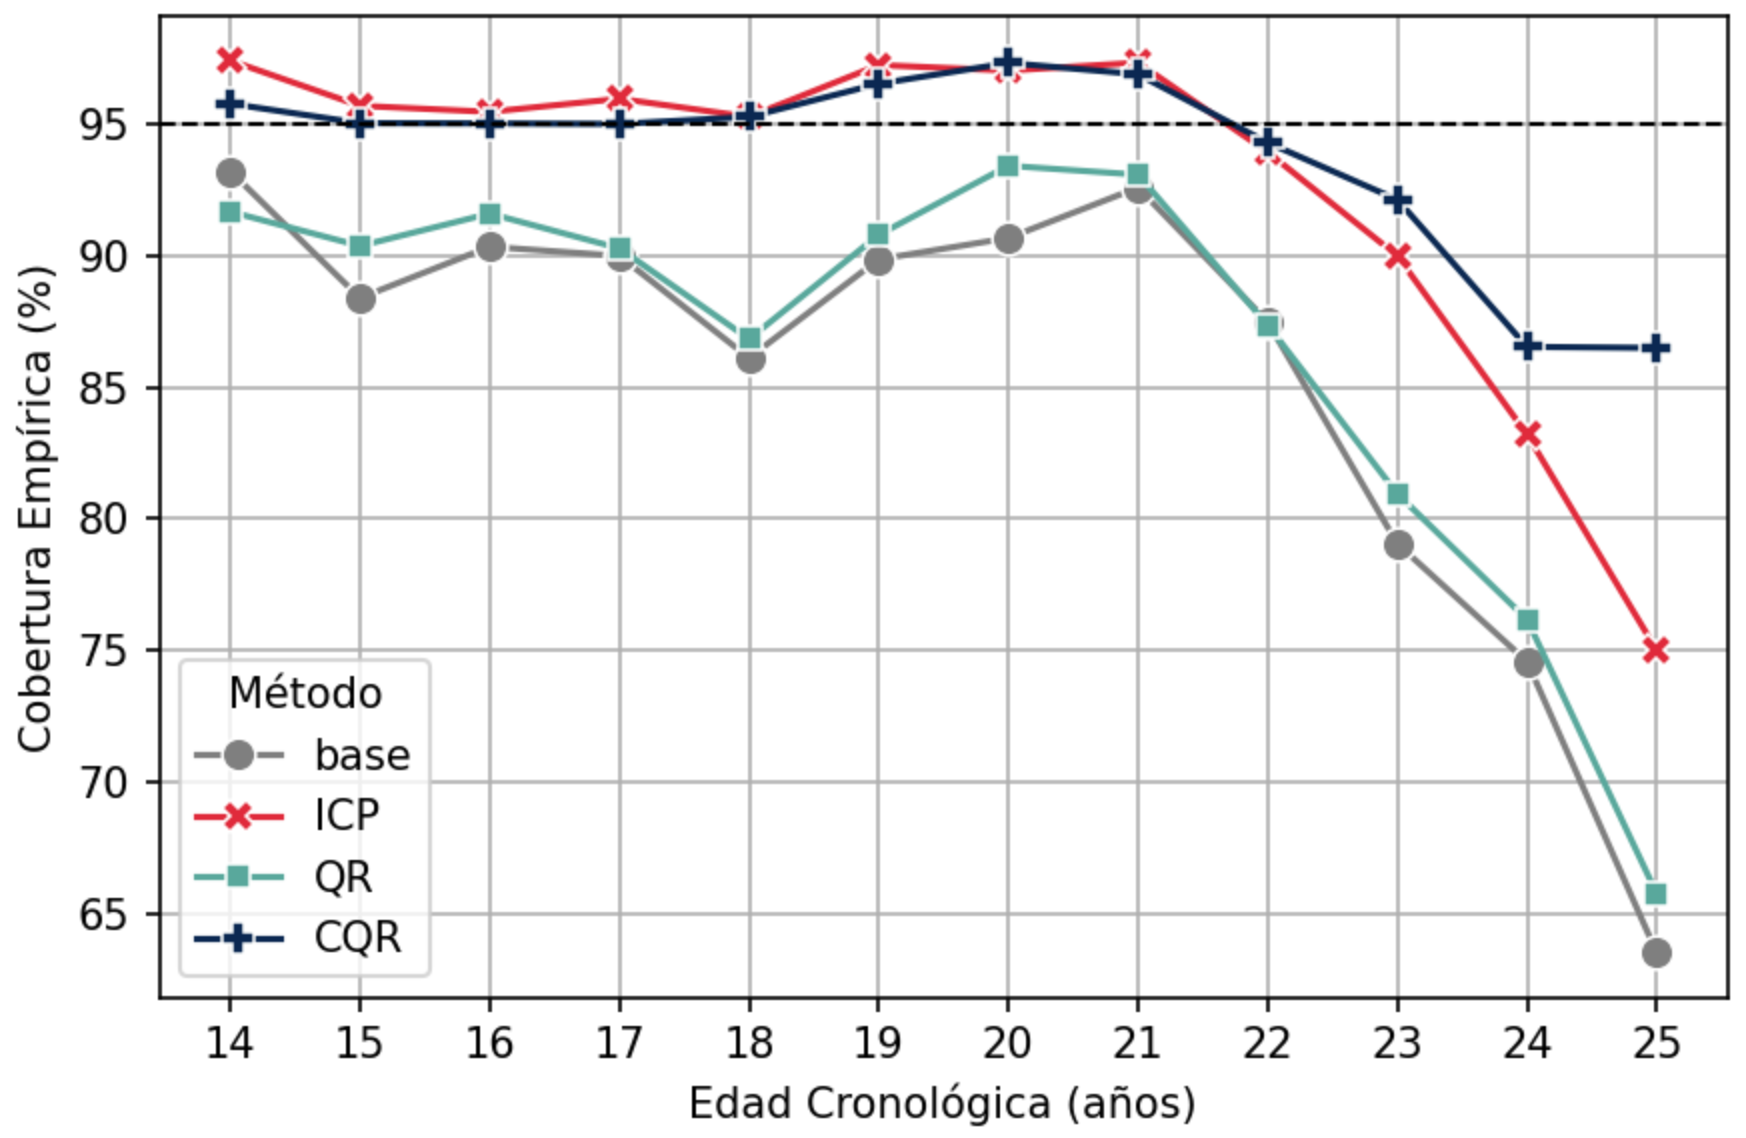
\includegraphics[width=\textwidth]{capitulos/cap_05/imagenes/AE_EC_by_true_age.png}
        \caption{
            Cobertura empírica del intervalo de predicción (\%) para cada método en función de la edad cronológica entera de los individuos. Se observa cómo varía la capacidad de cobertura según la edad y el método empleado.
        }
        \label{fig:AE_EC_by_true_age}
    \end{subfigure}

    \vspace{0.5cm}
    
    \begin{subfigure}[b]{0.9\textwidth}
        \centering
        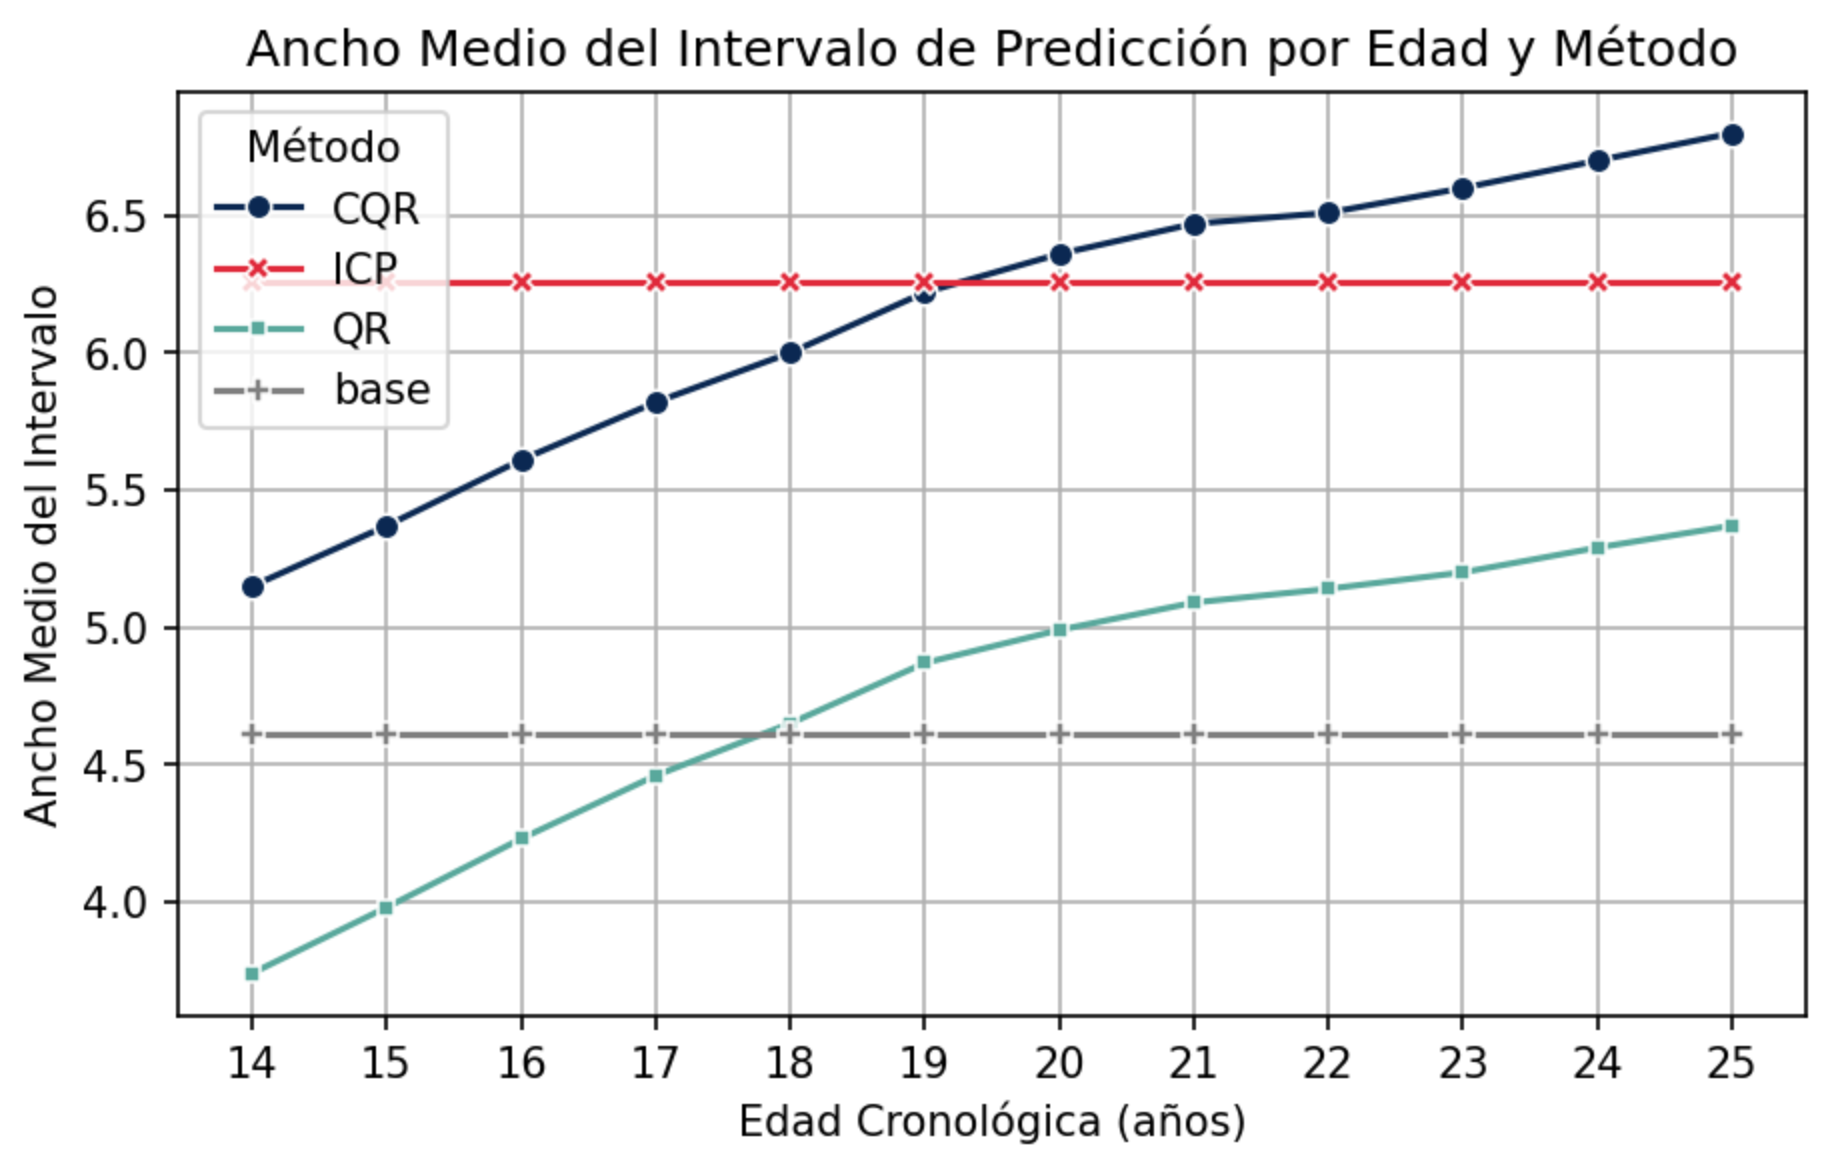
\includegraphics[width=\textwidth]{capitulos/cap_05/imagenes/AE_MPIW_by_true_age.png}
        \caption{
            Ancho medio del intervalo de predicción para cada método en función de la edad cronológica entera. Esta gráfica muestra cómo cambia la incertidumbre del modelo con la edad.
        }
        \label{fig:AE_MPIW_by_true_age}
    \end{subfigure}

    \caption[
        Análisis comparativo de la cobertura empírica y el ancho medio del intervalo de predicción por edad cronológica para los diferentes métodos evaluados.
    ]{
        Análisis comparativo de la cobertura empírica y el ancho medio del intervalo de predicción por edad cronológica para los diferentes métodos evaluados.
    }
    \label{fig:AE_EC_MPIW_by_true_age}
\end{figure}

\FloatBarrier

% ------------------------------------------------------------------------------------------------------------

\subsection{Resultados para la estimación de mayoría de edad}

\subsubsection{Análisis de métricas para la estimación de mayoría de edad puntual}

\begin{table}[h]
    \small
    \centering
    \begin{tabular}{ccccc}
    \toprule
    \multirow{2}{*}{\textbf{Método}} &  & \multicolumn{3}{c}{\textbf{\begin{tabular}[c]{@{}c@{}}Exactitud\\ (\%)\end{tabular}}} \\ \cline{3-5} 
                                    &  & \textbf{base}               & \textbf{LAC}               & \textbf{MCM}               \\ \cline{1-1} \cline{3-5} 
    Ejecución 1                      &  & 87.87                       & 86.99                      & 86.99                      \\
    Ejecución 2                      &  & 87.87                       & 87.36                      & 87.36                      \\
    Ejecución 3                      &  & 87.59                       & 86.52                      & 86.52                      \\
    Ejecución 4                      &  & 87.59                       & 87.5                       & 87.5                       \\
    Ejecución 5                      &  & 87.64                       & 87.13                      & 87.13                      \\
    Ejecución 6                      &  & 87.27                       & 86.71                      & 86.71                      \\
    Ejecución 7                      &  & 88.06                       & 87.13                      & 87.13                      \\
    Ejecución 8                      &  & 87.41                       & 86.2                       & 86.2                       \\
    Ejecución 9                      &  &                             &                            &                            \\
    Ejecución 10                     &  &                             &                            &                            \\ \cline{1-1} \cline{3-5} 
    Media                            &  & 0.88                        & 0.87                       & 0.87                       \\ 
    \bottomrule
    \end{tabular}
    \caption[
        Exactitud (\textit{accuracy}) obtenida por cada método de predicción a lo largo de las distintas ejecuciones. 
    ]{   
        Exactitud (\textit{accuracy}) obtenida por cada método de predicción a lo largo de las distintas ejecuciones. 
        Se presenta el valor para cada ejecución individual, así como la media final de la métrica.
        Punto como separador decimal.
    }
    \label{tab:AMM_accuracy_comparative}
\end{table}


\FloatBarrier


\subsubsection{Análisis de métricas para la estimación de mayoría de edad en conjunto de predicción}

\begin{table}[h]
    \small
    \centering
    \begin{tabular}{ccccccccc}
    \toprule
    \multirow{2}{*}{\textbf{Método}} &  & \multicolumn{3}{c}{\textbf{\begin{tabular}[c]{@{}c@{}}Cobertura \\[-0.8ex] Empírica (\%)\end{tabular}}} &  & \multicolumn{3}{c}{\textbf{\begin{tabular}[c]{@{}c@{}}Tamaño Medio \\[-0.8ex] del Conjunto\end{tabular}}} \\ \cline{3-5} \cline{7-9} 
                                    &  & \textbf{base}                   & \textbf{LAC}                  & \textbf{MCM}                  &  & \textbf{base}                   & \textbf{LAC}                   & \textbf{MCM}                   \\ \cline{1-1} \cline{3-5} \cline{7-9} 
    Ejecución 1                      &  & 87.87                           & 94.80                         & 93.91                         &  & 1                               & 1.20                           & 1.19                           \\
    Ejecución 2                      &  & 87.87                           & 95.07                         & 94.38                         &  & 1                               & 1.20                           & 1.21                           \\
    Ejecución 3                      &  & 87.59                           & 95.12                         & 94.24                         &  & 1                               & 1.23                           & 1.23                           \\
    Ejecución 4                      &  & 87.59                           & 93.96                         & 94.42                         &  & 1                               & 1.19                           & 1.21                           \\
    Ejecución 5                      &  & 87.64                           & 94.05                         & 93.54                         &  & 1                               & 1.18                           & 1.19                           \\
    Ejecución 6                      &  & 87.27                           & 93.96                         & 93.63                         &  & 1                               & 1.18                           & 1.20                           \\
    Ejecución 7                      &  & 88.06                           & 94.10                         & 93.87                         &  & 1                               & 1.19                           & 1.20                           \\
    Ejecución 8                      &  & 87.41                           & 94.89                         & 94.84                         &  & 1                               & 1.21                           & 1.22                           \\
    Ejecución 9                      &  &                                 &                               &                               &  &                                 &                                &                                \\
    Ejecución 10                     &  &                                 &                               &                               &  &                                 &                                &                                \\ \cline{1-1} \cline{3-5} \cline{7-9} 
    Media                            &  & 87.66                           & 94.49                         & 94.1                          &  & 1                               & 1.2                            & 1.2                            \\ \hline
    \end{tabular}
    \caption[
        Cobertura empírica y tamaño medio del conjunto de predicción obtenidos por cada método de predicción a lo largo de las distintas ejecuciones.
    ]{   
        Cobertura empírica y tamaño medio del conjunto de predicción obtenidos por cada método de predicción a lo largo de las distintas ejecuciones. 
        Se presentan los valores para cada ejecución individual, así como la media final de cada métrica. 
        Punto como separador decimal.
    }
    \label{tab:AMM_EC_MPSS_comparative}
\end{table}



\begin{figure}[h]
    \centering
    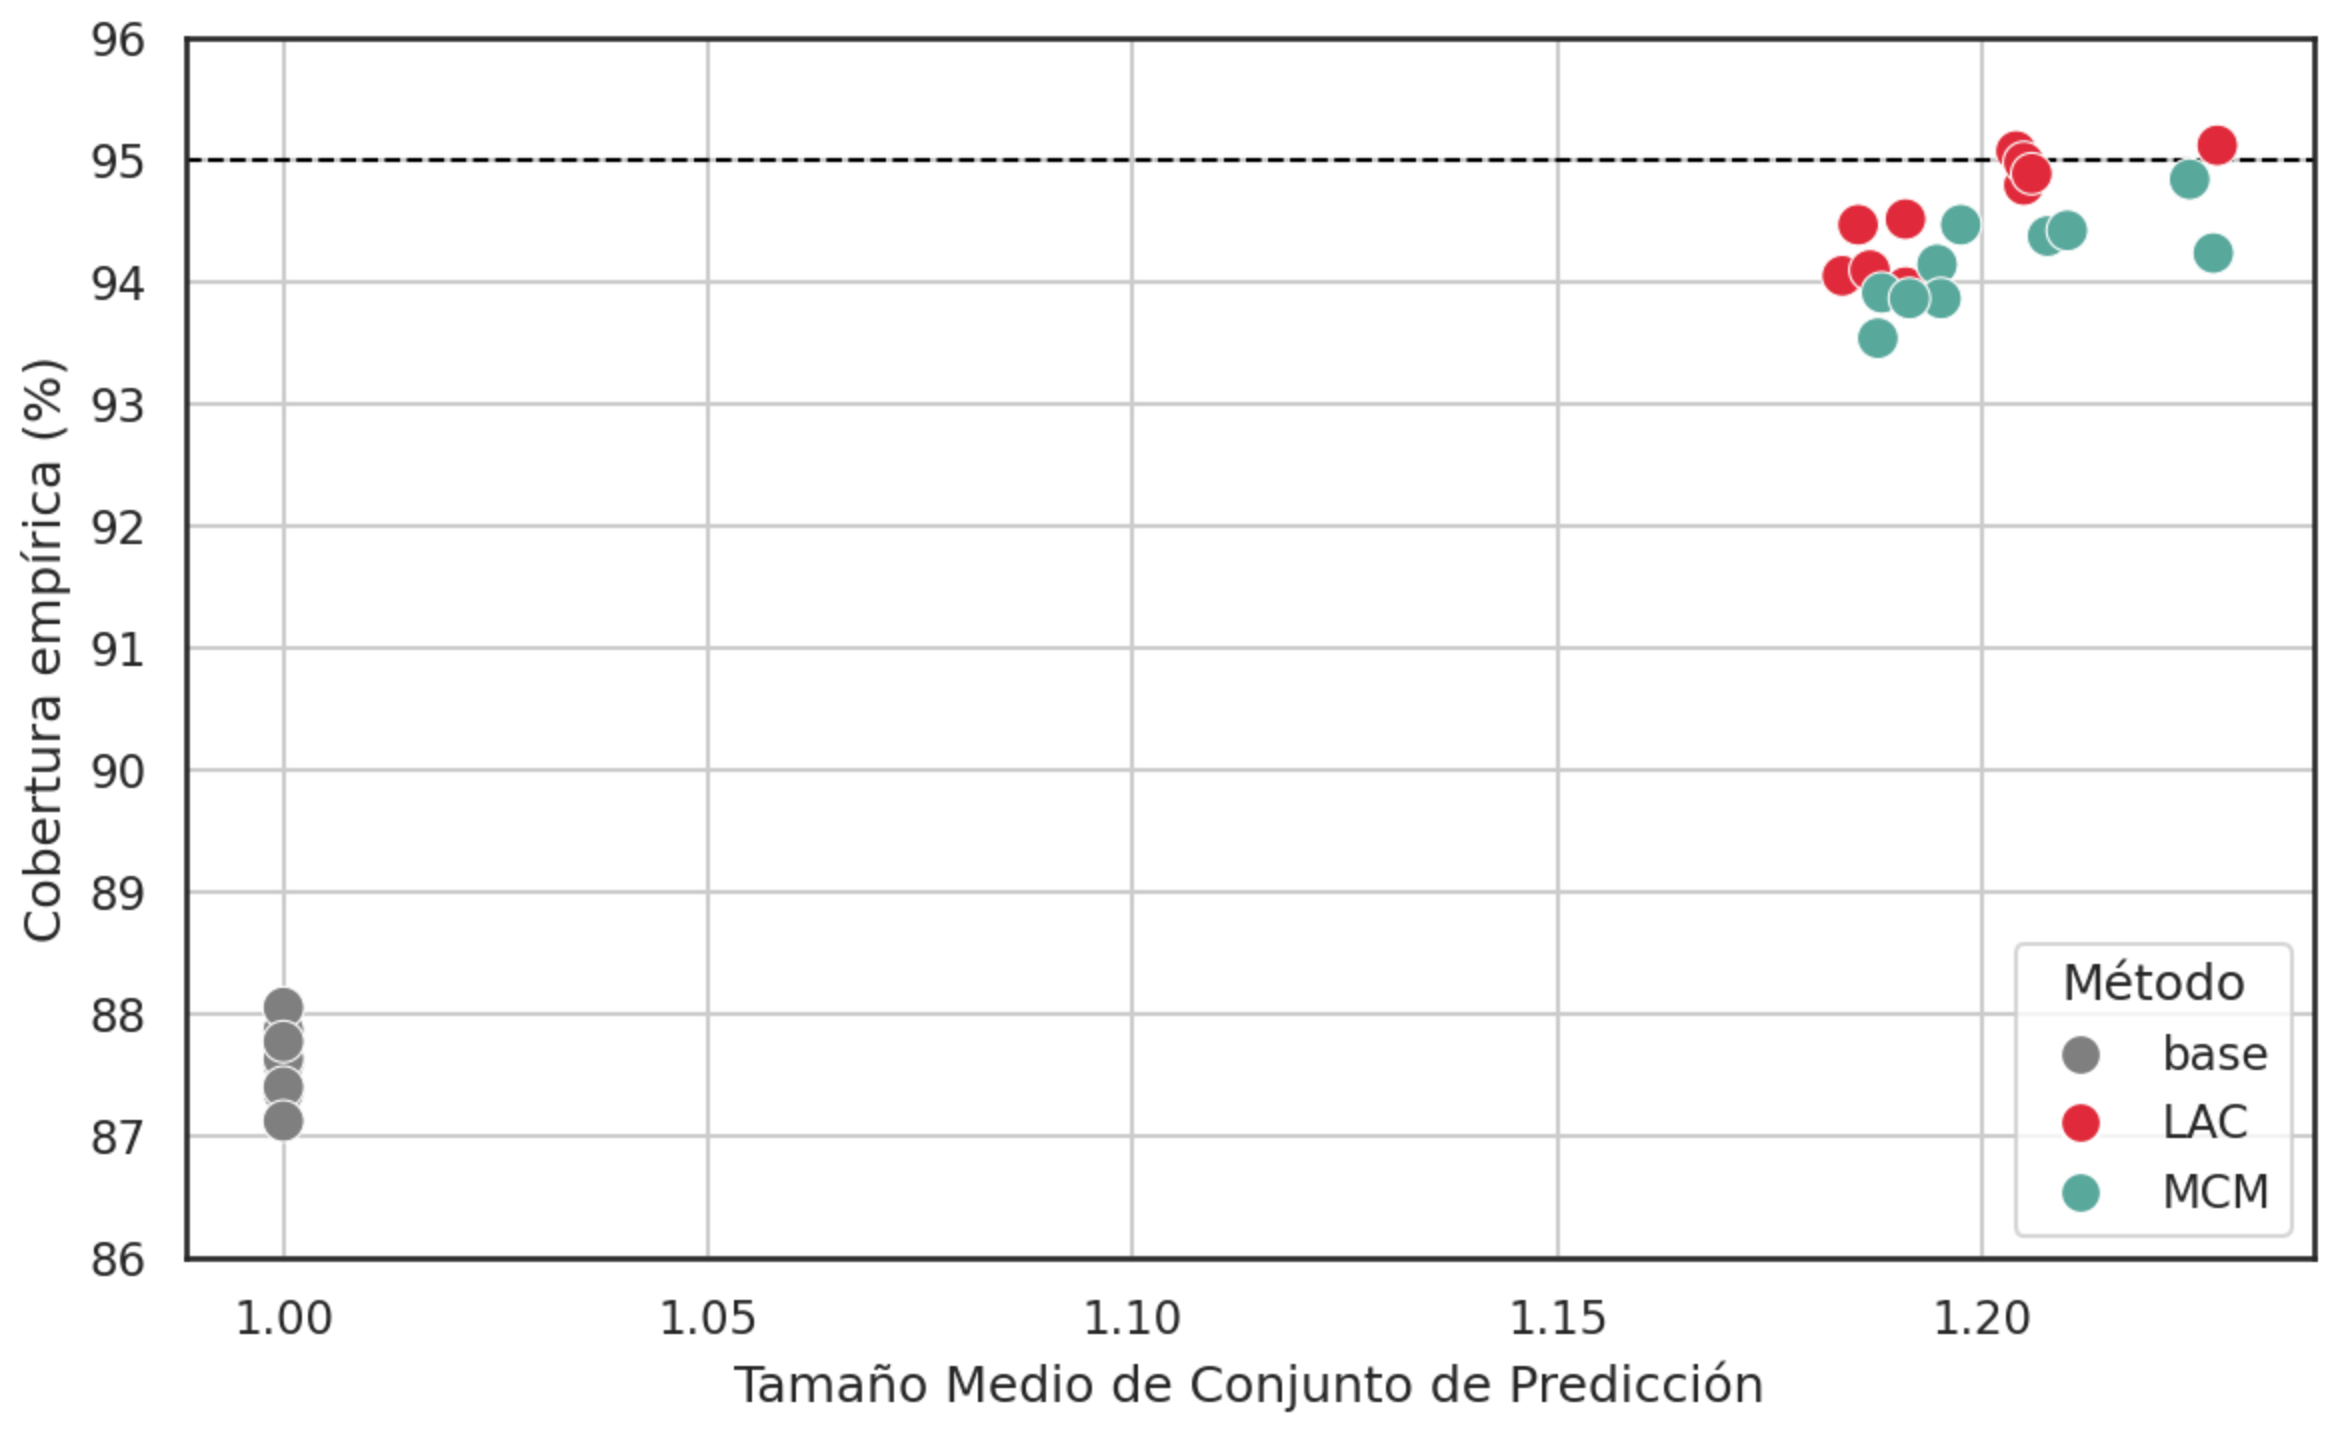
\includegraphics[width=\textwidth]{capitulos/cap_05/imagenes/AMM_scatterplot_EC-MPSS.png}
    \caption[
        Gráfica de dispersión \textit{Empirical Coverage}-\textit{Mean Prediction Set Size}
    ]{
        Gráfica de dispersión \textit{Empirical Coverage}-\textit{Mean Prediction Set Size}. 
    }
    \label{fig:AMM_scatterplot_EC-MPSS}
\end{figure}

\FloatBarrier

\subsubsection{Análisis de la cobertura en base a la clase}

\todo{En este apartado se analizará la cobertura mediante matrices de confusión conformal}

\begin{figure}[htbp]
    \centering

    % Tabla 1
    \begin{subfigure}[b]{0.6\textwidth}
        \centering
        \begin{tabular}{cc|ccc|}
        \cline{3-5}
          &     & \multicolumn{3}{c|}{Conjunto predicho}                              \\ \cline{3-5} 
          &     & \multicolumn{1}{c|}{\{$<$18\}} & \multicolumn{1}{c|}{\{$\geq$18\}} & \{$<$18,$\geq$18\} \\ \hline
        \multicolumn{1}{|c|}{\multirow{2}{*}{\begin{tabular}[c]{@{}c@{}}Valor \\[-1.4ex] real\end{tabular}}} & $<$18 & \multicolumn{1}{c|}{738}   & \multicolumn{1}{c|}{115}   & 0         \\ \cline{2-5} 
        \multicolumn{1}{|c|}{} & $\geq$18 & \multicolumn{1}{c|}{142}   & \multicolumn{1}{c|}{1157}  & 0         \\ \hline
        \end{tabular}
        \caption{base}
    \end{subfigure}

    \vspace{1em} % Espacio vertical entre tablas

    % Tabla 2
    \begin{subfigure}[b]{0.6\textwidth}
        \centering
        \begin{tabular}{cc|ccc|}
        \cline{3-5}
          &     & \multicolumn{3}{c|}{Conjunto predicho}                              \\ \cline{3-5} 
          &     & \multicolumn{1}{c|}{\{$<$18\}} & \multicolumn{1}{c|}{\{$\geq$18\}} & \{$<$18,$\geq$18\} \\ \hline
        \multicolumn{1}{|c|}{\multirow{2}{*}{\begin{tabular}[c]{@{}c@{}}Valor \\[-1.4ex] real\end{tabular}}} & $<$18 & \multicolumn{1}{c|}{567}   & \multicolumn{1}{c|}{58}   & 228         \\ \cline{2-5} 
        \multicolumn{1}{|c|}{} & $\geq$18 & \multicolumn{1}{c|}{48}   & \multicolumn{1}{c|}{1040}  & 211         \\ \hline
        \end{tabular}
        \caption{LAC}
    \end{subfigure}

    \vspace{1em}

    % Tabla 3
    \begin{subfigure}[b]{0.6\textwidth}
        \centering
        \begin{tabular}{cc|ccc|}
        \cline{3-5}
            &     & \multicolumn{3}{c|}{Conjunto predicho}                              \\ \cline{3-5} 
            &     & \multicolumn{1}{c|}{\{$<$18\}} & \multicolumn{1}{c|}{\{$\geq$18\}} & \{$<$18,$\geq$18\} \\ \hline
        \multicolumn{1}{|c|}{\multirow{2}{*}{\begin{tabular}[c]{@{}c@{}}Valor \\[-1.4ex] real\end{tabular}}} & $<$18 & \multicolumn{1}{c|}{646}   & \multicolumn{1}{c|}{28}   & 179         \\ \cline{2-5} 
        \multicolumn{1}{|c|}{} & $\geq$18 & \multicolumn{1}{c|}{83}   & \multicolumn{1}{c|}{912}  & 304         \\ \hline
        \end{tabular}
        \caption{MCM}
    \end{subfigure}

    \caption[
        Matrices de confusión conformal correspondientes a tres modelo de `base', LAC y MCM.
    ]{
        Matrices de confusión conformal correspondientes a tres modelo de `base', LAC y MCM.
    }
    \label{fig:conf2matrix}
\end{figure}

\FloatBarrier

% ------------------------------------------------------------------------------------------------------------

\subsection{Resultados para la clasificación combinada de sexo y mayoría de edad}


\subsubsection{Análisis de métricas para la clasificación se sexo y mayoría de edad}



\begin{table}[h]
    \small
    \centering
    \begin{tabular}{ccccccccccccc}
    \toprule
    \multirow{2}{*}{\textbf{Método}} &  & \multicolumn{5}{c}{\textbf{\begin{tabular}[c]{@{}c@{}}Cobertura \\[-0.8ex] empírica (\%)\end{tabular}}} &  & \multicolumn{5}{c}{\textbf{\begin{tabular}[c]{@{}c@{}}Tamaño Medio \\[-0.8ex] del Conjunto\end{tabular}}} \\ \cline{3-7} \cline{9-13} 
    &  & \textbf{base} & \textbf{LAC} & \textbf{MCM} & \textbf{APS} & \textbf{RAPS} &  & \textbf{base} & \textbf{LAC} & \textbf{MCM} & \textbf{APS} & \textbf{RAPS} \\ \cline{1-1} \cline{3-7} \cline{9-13} 
    Ejecución 1 &  & 77.79 & 94.47 & 95.26 & 95.72 & 97.58 &  & 1 & 1.79 & 1.9 & 2.32 & 2.49 \\
    Ejecución 2 &  & 76.49 & 95.07 & 94.8 & 95.45 & 97.68 &  & 1 & 1.86 & 1.89 & 2.28 & 2.45 \\
    Ejecución 3 &  & 76.35 & 93.77 & 93.4 & 94.56 & 96.61 &  & 1 & 1.91 & 1.9 & 2.35 & 2.52 \\
    Ejecución 4 &  & 75.23 & 94.75 & 94.8 & 94.7 & 96.84 &  & 1 & 1.89 & 1.9 & 2.34 & 2.48 \\
    Ejecución 5 &  & 74.95 & 93.68 & 93.82 & 95.59 & 97.44 &  & 1 & 1.71 & 1.76 & 2.33 & 2.55 \\
    Ejecución 6 &  & 77.04 & 93.4 & 93.49 & 95.72 & 97.17 &  & 1 & 1.83 & 1.99 & 2.38 & 2.52 \\
    Ejecución 7 &  & 76.07 & 93.49 & 93.73 & 95.49 & 97.26 &  & 1 & 1.78 & 1.84 & 2.4 & 2.57 \\
    Ejecución 8 &  & 74.44 & 94.01 & 94.42 & 95.54 & 97.35 &  & 1 & 1.79 & 1.82 & 2.3 & 2.51 \\
    Ejecución 9 &  &  &  &  &  &  &  &  &  &  &  &  \\
    Ejecución 10 &  &  &  &  &  &  &  &  &  &  &  &  \\ \cline{1-1} \cline{3-7} \cline{9-13} 
    Media &  & \multicolumn{1}{r}{76.05} & 94.08 & 94.21 & \multicolumn{1}{r}{95.35} & \multicolumn{1}{r}{97.24} &  & 1 & 1.82 & \multicolumn{1}{r}{1.87} & 2.34 & 2.51 \\ 
    \bottomrule
    \end{tabular}
    \caption[
        Cobertura empírica y tamaño medio del conjunto de predicción obtenidos por cada método de predicción a lo largo de las distintas ejecuciones.
    ]{   
        Cobertura empírica y tamaño medio del conjunto de predicción obtenidos por cada método de predicción a lo largo de las distintas ejecuciones. Se presentan los valores para cada ejecución individual, así como la media final de cada métrica. 
        Punto como separador decimal.
    }
    \label{tab:AMSC_EC_MPSS_comparative}
\end{table}

Probablemente MCM empeore a LAC por la menor cantidad de datos a emplear para la calibración (ya que los datos se dividen en cuatro subconjunto dependiendo de la clase a calibrar)



\subsubsection{Análisis de la cobertura en base a la clase}

\todo{He pensado en utilizar un diagrama de Venn de 4 conjuntos (1 por cada clase) a modo de matriz de confusión conformal}


% ------------------------------------------------------------------------------------------------------------

%\subsection{Resultados para la estimación de edad como problema de clasificación}



% ------------------------------------------------------------------------------------------------------------
% ------------------------------------------------------------------------------------------------------------


